\documentclass{book}

\usepackage{cite}
\usepackage{amsmath,amssymb,amsfonts}
\usepackage{algorithmic}
\usepackage{graphicx}
\usepackage{textcomp}
\usepackage{xcolor}

\graphicspath{{Images/}}


\usepackage{csquotes}
\usepackage{mdframed}

\usepackage{listings}
\usepackage{float}
\usepackage{array}
\usepackage{booktabs}
\usepackage{enumitem}
\usepackage{hyperref}
\usepackage{multirow}
\usepackage{pgfplots}
\pgfplotsset{compat=1.8}

\usepackage{csquotes}
\usepackage{mdframed}


\newcommand{\signatureSlot}[1]{
\vspace{3em}
\begin{tabular}{r p{2in}}
#1: & \hrulefill \\
\end{tabular}
\vspace{2em}}

\newcommand{\TASignatureSlot}{
\refstepcounter{TASignatures}
\signatureSlot{TA Signature \arabic{TASignatures}}
}
\newcounter{TASignatures}




%for including code in the document
\usepackage{listings}
\usepackage{xcolor}
\definecolor{codegreen}{rgb}{0,0.6,0}
\definecolor{codegray}{rgb}{0.5,0.5,0.5}
\definecolor{codepurple}{rgb}{0.58,0,0.82}
\definecolor{backcolour}{rgb}{0.95,0.95,0.92}

\lstdefinestyle{mystyle}{
    backgroundcolor=\color{backcolour},   
    commentstyle=\color{codegreen},
    keywordstyle=\color{magenta},
    numberstyle=\tiny\color{codegray},
    stringstyle=\color{codepurple},
    basicstyle=\ttfamily\footnotesize,
    breakatwhitespace=false,         
    breaklines=true,                 
    captionpos=b,                    
    keepspaces=true,                 
    numbers=left,                    
    numbersep=5pt,                  
    showspaces=false,                
    showstringspaces=false,
    showtabs=false,                  
    tabsize=2
}

%Macro used to insert an aside into the lab manual
\newcommand{\aside}[1]{
\refstepcounter{AsideCounter}
\begin{samepage}
\begin{center}
\begin{displayquote}
\begin{mdframed}
\textit{|Note \arabic{AsideCounter}| #1}
\end{mdframed}
\end{displayquote}
\end{center}
\end{samepage}
}
\newcounter{AsideCounter}

\newcommand{\rungincondition}{rung-condition-in}
\newcommand{\rungoutcondition}{rung-condition-out}

\newcommand{\comment}[1]{}

\renewcommand*{\figureautorefname}{Fig.}


\newcommand{\us}{\textunderscore}

\title{Introduction to PLC Automation}
\newcommand{\booksubtitle}{Practical Excercises}
\newcommand{\booklicense}{CC BY-SA 4.0}


\author{Dr. Jesse Roberts}
% Author subtitle could be a university or a geographical location, for example
\newcommand{\authorsubtitle}{Cookeville, TN}

% Create convenient commands \booktitle and \bookauthor
\makeatletter
\newcommand{\booktitle}{\@title}
\newcommand{\bookauthor}{\@author}
\makeatother


% This utf8 declaration is not needed for versions of latex > 2018 but may
% be helpful for older software. Eventually it may not be worth keeping.
\usepackage[utf8]{inputenc}  
\usepackage{fix-cm}  % this package allows large \fontsize
\usepackage{tikz}    % this is for graphics. e.g. rectangle on title page
\usepackage{amsmath} % Used by equations

% The following dimensions specify 4.75" X 7.5" content on 6 3/8" by 9 1/4"
% paper. The paper width and height can be tweaked as required and the content
% should size to fit within the margins accordingly.
%
% The (inside) bindingoffset should be larger for books with more pages. Some
% standard recommended sizes are .375in minimum up to 1in for 600+ page books.
% Sizes .75in and .875in are also recommended roughly at 150 and 400 pages.
\usepackage[bindingoffset=0.625in,
            left=.5in, right=.5in,
            top=.8125in, bottom=.9375in,
            paperwidth=6.375in, paperheight=9.25in]{geometry}
% Here is an alternative geometry for reading on letter size paper:
% \usepackage[margin=.75in, paperwidth=8.5in, paperheight=11in]{geometry}

\renewcommand{\contentsname}{Table of Contents} % default is {Contents}
\usepackage{makeidx}
\makeindex % Initialize an index so we can add entries with \index


% Content Starts Here
\begin{document}
\frontmatter

% % ---- Half Title Page ----
% % current geometry will be restored after title page
% \newgeometry{top=1.75in,bottom=.5in}
% \begin{titlepage}
% \begin{flushleft}

% % Title
% \textbf{\fontfamily{qcs}\fontsize{48}{54}\selectfont Introduction \\ to PLC \\ \vskip6pt Automation}

% % Draw a line 4pt high
% \par\noindent\rule{\textwidth}{4pt}\\

% % Subtitle
% % Shaded box from left to right. Text node is midway (centered).
% \begin{tikzpicture}
% \shade[bottom color=lightgray,top color=white]
%     (0,0) rectangle (\textwidth, 1.5)
%     node[midway] {\textbf{\large \textit{\booksubtitle}}};
% \end{tikzpicture}

% % Edition Number
% \begin{flushright}
% \Large First Edition
% \end{flushright}

% % \vspace{\fill}
% \vspace{\fill}

% \end{flushleft}
% \end{titlepage}
% \restoregeometry
% % ---- End of Half Title Page ----


% % No page numbers on the Frontispiece page
% \thispagestyle{empty}


% ---- Title Page ----
% current geometry will be restored after title page
\newgeometry{top=1.75in,bottom=.5in}
\begin{titlepage}
\begin{flushleft}

% Title
\textbf{\fontfamily{qcs}\fontsize{48}{54}\selectfont Introduction \\ to PLC \\ \vskip6pt Automation}

% Draw a line 4pt high
\par\noindent\rule{\textwidth}{4pt}\\

% Shaded box from left to right with Subtitle
% The text node is midway (centered).

\begin{tikzpicture}
\shade[bottom color=lightgray,top color=white]
    (0,0) rectangle (\textwidth, 1.5)
    node[midway] {\textbf{\large \textit{\booksubtitle}}};
\end{tikzpicture}

% Edition Number
\begin{flushright}
\Large First Edition
\end{flushright}

\vspace{\fill}

% Author and Location
\textbf{\large \bookauthor}\\[3.5pt]
\textbf{\large \textit{\authorsubtitle}}

\vspace{\fill}

% Self Publishing Logo. Free to use: CC0 license.
% The source file is book.svg. If you change the svg, you must then convert
% it to pdf. There are many online and offline tools available to do that.
\begin{center}

\includegraphics{booksvg.pdf}\\[4pt]
\fontfamily{lmtt}\small{Self Publishers Worldwide\\
Seattle San Francisco New York\\
London Paris Rome Beijing Barcelona}
\end{center}

\end{flushleft}
\end{titlepage}
\restoregeometry
% ---- End of Title Page ----

% Do not show page numbers on colophon page
\thispagestyle{empty}

\begin{flushleft}
\vspace*{\fill}
This book was typeset using \LaTeX{} software.\\
\vspace{\fill}
Copyright \textcopyright{} \the\year{}  \bookauthor\\
License: \booklicense
\end{flushleft}

% A title page resets the page # to 1, but the second title page
% was actually page 3. So add two to page counter.
\addtocounter{page}{2}

% The asterisk excludes chapter from the table of contents.
\chapter*{Preface}

This book is a collection of exercises that are based on real scenarios and problems frequently encountered in industrial automation. The exercises are intended to be completed after having watched the associated video lecture available \href{https://www.youtube.com/watch?v=DroUeHOe4lw&list=PL08zDkmLSnzFXJt9FVlfNPbG_KlcI_Qck&pp=gAQBiAQB}{here}. 

Each exercise has an associated starter file. The collection of starter files can be found \href{https://github.com/JesseTNRoberts/Introduction-to-PLC-Automation/}{here}.

The first chapter is first exercise in this book and details the process of downloading a program to the PLC and HMI and then performing edits to those programs. This chapter will likely need to be referred to at the beginning of many exercises. However, rather than repeating the instructions, readers are expected to refer to the first chapter (Lab 0) as necessary for download process details.

% Three-level Table of Contents
\setcounter{tocdepth}{3}
\tableofcontents

\mainmatter

\chapter{Lab 0}
\setcounter{TASignatures}{0}
\setcounter{AsideCounter}{0}

\section{Introduction}
    \vspace{0.1em}

    \textbf{In this lab you gain experience with:}
    \begin{enumerate}
        \item How to download project files to the PLC
        \item How to download applications to the HMI
        \item How to make online edits to the ladder program
        \item How to make offline edits to the ladder program
        \item How to toggle a bit
    \end{enumerate}
    
    \vspace{1em}
    \textbf{In this lab you will be exposed to:}
    \begin{enumerate}
        \item Ladder logic
        \item Logical OR and Logical AND
        \item Normally closed contact (XIO)
        \item Normally open contact (XIC)
        \item Output coil (OTE)
    \end{enumerate}
    
\subsection{How to get credit}
Each lab after this will require each student to submit the completed pre-lab before they are allowed to begin working on the lab. The \textbf{pre-lab must be submitted to the TA before beginning work on the lab}. If it is not complete then you will be required to complete the pre-lab before you are allowed to begin working on the lab.

In order to get credit for completing each part of this lab, \textbf{you must personally read and complete each portion of the lab and demonstrate the completion to the TA}. Each section has one or more signature slots that must be signed by the TA to confirm that the section was completed. Each section is worth equal credit. 

\subsection{20 minute grace period}
To receive full credit, the lab must be completed and demonstrated during the assigned lab time. However, if you cannot complete the lab within that time, you can complete and demonstrate the lab within the first 20 minutes of the subsequent lab time and still receive full credit. \textbf{If the lab is not completed within the assigned lab time and is not completed within the 20 minute grace period, then the lab is considered late}. If you submit the lab late, then there will be a 20\% deduction compounded weekly.


\subsection{Safety}

The PLCs and equipment in this lab use \textbf{120VAC and 24VDC}. The equipment is considered finger safe, which means that accidental contact with the electrical circuitry is \textit{unlikely}. However, there are small gaps around the connections to the PLC and other equipment which expose small portions of bare wires or bare metal from the bussbars. 
\\
\textbf{DO NOT TOUCH ANY BARE WIRES or METAL EXPOSED AROUND BUSSBARS! YOU WILL BE SHOCKED!}
\\

\subsection{Lab agreement}

The planning of a program is often a very social activity, however the actual writing of the code is always an individual pursuit. In this class it is very much the same. Students are welcome to verbally assist each other, but each person is required to write their own code and personally complete each lab. In this way each student will gain valuable experience with programming PLCs. 

\textbf{The undersigned person guarantees that any and all work demonstrated to the TA in regard to this lab is a result of their own work with no unauthorized help. Further, they acknowledge all course and safety information which has been given.}

\signatureSlot{Student (Print \& Sign)}


\section{Downloading to the PLC}

In this section you will download the Lab 0 project to the programmable logic controller (PLC). Be careful not to \textbf{mix up downloading and uploading}. Downloading is pushing code into the PLC. Uploading is pulling the code from the PLC into the computer. In this class you should \textbf{never upload}. 

The code that is in the PLC when you arrive to the lab is most likely not the code that you left in it from the previous lab. So, make sure that you save your lab progress to the lab drive or to a flash drive for safe keeping. 

This section serves as \textbf{general instructions for downloading to the PLC}. Refer to this lab manual in future labs if you forget how to download to the PLC.

\subsection{Get the lab files from iLearn}

In this lab you will often be working with a pre-made lab PLC and HMI file. As the semester progresses this will change. However, for the next several labs you will need to logon to ilearn and download the necessary lab files to the lab PC at the beginning of lab. Download all the files in the Lab0 ilearn folder under content now.

\subsection{Open Studio 5000}

Studio 5000 is the development environment used to modify Allen Bradley PLC ladder logic and download to the PLC. To open the program, click the windows icon in the bottom left and navigate to a folder called \textbf{Rockwell Software}. Open the folder and select \textbf{Studio 5000}. This will launch the software.

A splash screen like the one in \figureautorefname \ref{fig:SplashScreen} should appear. Select \textbf{Existing Project}. From the drop down that appears, select the option that says \textbf{Project File}. Navigate to the Lab PLC project that was downloaded from iLearn and select the file, then click \textbf{Open}.

\begin{figure}[h]
\centering
\textbf{Studio 5000 Splash Screen}\par \medskip
\frame{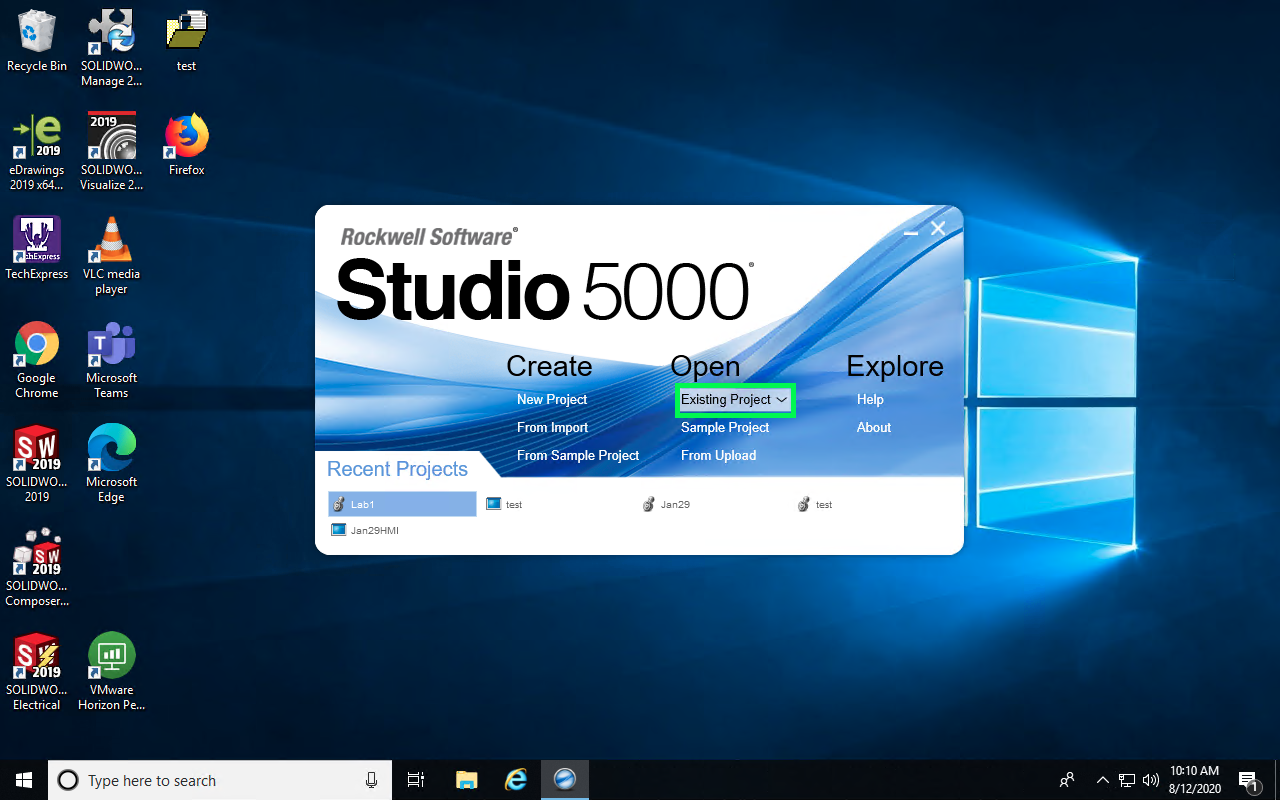
\includegraphics[width=3.2in]{Studio5000SplashScreen}}
\caption{Studio 5000}
\label{fig:SplashScreen}
\end{figure}

\subsection{Set the project path}

Now that Studio 5000 has been launched and the appropriate Lab project has been opened, you have to point Studio 5000 at the PLC which you will be using. This is referred to as setting the project path. \textbf{This is a very important step!}. Your classmates and TA will not be happy with you if you do not perform this step correctly, as it will cause you to \textbf{download to someone else's PLC}. 

\aside{Accidents happen and you will be forgiven for accidentally downloading to the wrong PLC. This happens to professionals as well. However, if the TA believes that you did this intentionally, \textbf{you may be asked to leave the lab}.}

\subsubsection{What is setting the project path?}
PLCs on a network are identified by their internet protocol (IP) address. The IP address for each of the PLCs in this lab corresponds with the lab seat number. Refer to \tableautorefname \ref{Table:PLCIpAddresses} to identify which PLC IP address corresponds with your seat number.

\textbf{Setting the project path is what Allen Bradley calls choosing the IP address of the PLC to which you will download code}.

\begin{table}[h]
\centering
\caption{PLC IP addresses}
\label{Table:PLCIpAddresses}
\begin{tabular}{c l | c l}
\toprule
Seat \# & IP Address & Seat \# & IP Address\\
\midrule
1 & $192.168.100.201$ & 2 & $192.168.100.202$ \\
3 & $192.168.100.203$ & 4 & $192.168.100.204$ \\
5 & $192.168.100.205$ & 6 & $192.168.100.206$ \\
7 & $192.168.100.207$ & 8 & $192.168.100.208$ \\
9 & $192.168.100.209$ & 10 & $192.168.100.210$ \\
11 & $192.168.100.211$ & 12 & $192.168.100.212$ \\
\bottomrule
\end{tabular}
\end{table}

\subsubsection{How do you set the project path?}

To set the project path, select the item in the menu bar called \textbf{Communications}. From the drop down, select \textbf{Who Active}. Here is where you will choose the PLC project path. Scroll to the PLC with the IP address associated with your seat and click the PLC to highlight it. Then select \textbf{Set Project Path}. 

\aside{If after highlighting the PLC, the option to set project path is still grayed out then you have either not selected the correct item or the project path is already pointing at your PLC. }

There is a plus icon beside the PLC that allows you to view items associated with that particular PLC. However, to set the project path you must select the outer most object. If this is confusing, refer to \figureautorefname \ref{fig:WhoActive}.


\begin{figure}[h]
\centering
\textbf{Who Active}\par \medskip
\frame{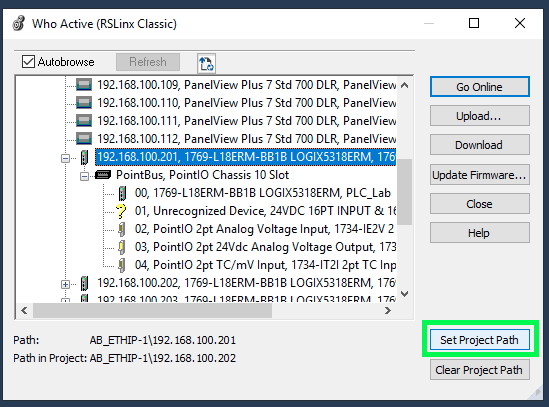
\includegraphics[width=3.2in]{WhoActive}}
\caption{Who Active}
\label{fig:WhoActive}
\end{figure}

\aside{In \figureautorefname \ref{fig:WhoActive} the user was sitting in seat number 1. \textbf{You most likely will not select the same PLC IP address shown in the image.} Refer to \tableautorefname \ref{Table:PLCIpAddresses} to verify which IP address is associated with your seat.}


\textbf{Do not select any other option other than Set Project Path!} After setting the project path, the option will be greyed out. Close the dialog window after setting the project path.

\subsection{Download to the PLC}
\label{subsection:DownloadPLC}

It is now time to download to the PLC. Again click the \textbf{Communications} option in the menu. From the dropdown, select \textbf{Download}. 

\aside{If the download option is grayed out, then you have either not set the project path or you are currently online with the PLC.} 

If you are online with the PLC, you will have to go to the Communications menu and select Go Offline before being able to Download.

\begin{figure}[h]
\centering
\textbf{Download Dialog}\par \medskip
\frame{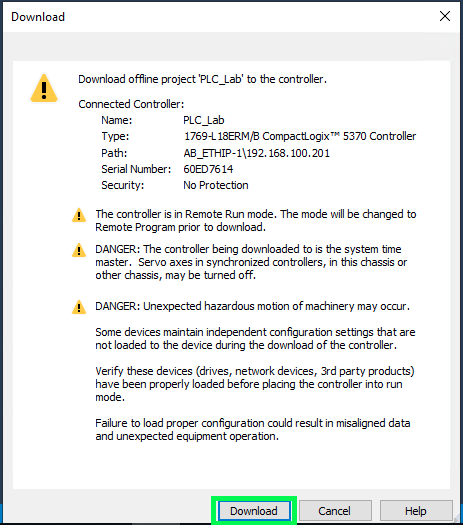
\includegraphics[width=3.2in]{DownloadMenu}}
\caption{Download dialog}
\label{fig:DownloadDialog}
\end{figure}

After selecting to download the code, a dialog window will appear. Click \textbf{Download} at the bottom of the dialog. For reference see \figureautorefname \ref{fig:DownloadDialog}.

\aside{In an industrial environment downloading can cause things to behave dangerously but in this lab environment we can ignore this warning.}

\aside{Before downloading the code to the PLC, Studio 5000 will automatically compile what you have written. If there is a compilation error, you will be informed and the download will be aborted.}


\subsection{Ensure that the PLC is in run mode}

After downloading the code to the PLC the code will not execute until the PLC is in run mode. Typically, after downloading to the PLC a dialog window will appear asking if you would like to return to run mode. Select, yes.

If for some reason the prompt does not appear, go to the Communications menu and select Go Online. Then go to the Communicaitons menu and select Run Mode.

\subsection{Open the Main Routine}

To view the code that is in the project, open the tasks dropdown in the left side menu. Here is where "routines" are kept. In each lab there will be a MainRoutine that houses the code. Refer to \figureautorefname \ref{fig:MainRoutine}. Double click the MainRoutine to open and view the code.

In \figureautorefname \ref{fig:TheCode} the code housed in MainRoutine is displayed. Notice there is a comment denoting the rung which you will be editing later in the lab. Also notice that the side bars of the "ladder" are green. This means that this code is currently "being scanned" or "being executed" by the PLC. If the PLC were not in run mode then the side bars would not be green. Also, if the user were not online with the PLC the side bars would not be green. 

\aside{The side bars being green is meant to signigy that they are energized. Ladder logic is intended to be read like an electrical schematic. Things that are green are energized. Notice that the \textbf{normally open contacts} associated with $Lab0.October$ and $Lab0.November$ are grey as is the \textbf{coil} associated with Lab0.Its\textunderscore Fall. This means that these are not energized.}

\begin{figure}[h]
\centering
\textbf{Tasks Dropdown}\par \medskip
\frame{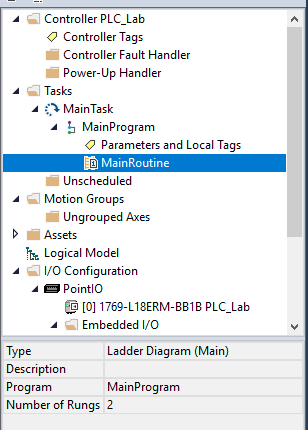
\includegraphics[width=3.2in]{MainRoutine}}
\caption{Tasks Dropdown and Main Routine}
\label{fig:MainRoutine}
\end{figure}


\begin{figure}[h]
\centering
\textbf{The Lab0 MainRoutine}\par \medskip
\frame{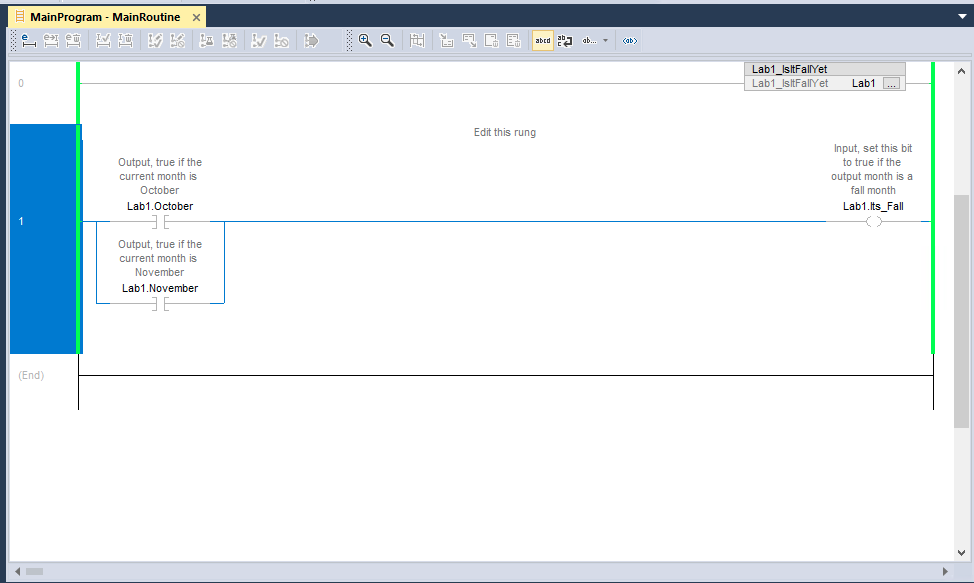
\includegraphics[width=3.2in]{Code}}
\caption{The code housed in the MainRoutine}
\label{fig:TheCode}
\end{figure}


\subsection{Go Online}
\label{subsection:GoOnline}

After downloading and ensuring that the PLC is in Run Mode, it is time to Go Online. Going online allows you to see the actual current state of the PLC and monitor the code as it executes. \textbf{Go to the communications menu and select Go Online}.

\aside{The code that is in Lab 0 is supposed to decide if it is Fall based on the month. However, you may notice that there is a logical error. We will fix this later on.}

\TASignatureSlot


\section{Downloading to the HMI}

PLCs work hand in hand with the human machine interface (HMI). The HMI is how operators are able to give input to and view the state of the machine. In this section you will learn how to restore an archived HMI application, generate a runtime application, and download the runtime application to the HMI.

\subsection{Open FactoryTalk View Studio}

The software used to edit HMI applications and download those applications to the HMI is called FactoryTalk View Studio. \textbf{Click the windows icon in the bottom left and navigate to FactoryTalk View Studio}. 

When the program launches, a dialog will appear asking if you would like to open an application or create a new application. The HMI files that we distribute cannot be opened through this dialog window. \textbf{Click cancel. This will close the dialog window}. 

\aside{To distribute HMI files they must be distributed as "backups". This is an odd idiosyncrasy of the FactoryTalk View Studio. These backups can't be opened through the initial dialog window. Rather, they must be "restored".}

\subsection{Restore the HMI application}

To restore the HMI application that you downloaded from iLearn, \textbf{go to the tools menu and select Application Manager}. This will open the FactoryTalk View ME Application Manager. This is actually a separate program that is launched. \textbf{Highlight the button beside Restore Application and click next}. 

You are then prompted for the location of the application archive. \textbf{Click the box with the three periods (ellipse) to open a file explorer windown}. Navigate to the application archive file downloaded from iLearn \textbf{open the file}. This will return you to the FactoryTalk View ME Application Manager Manager. \textbf{Click next}.

You are now prompted for a name to be given to the application. \textbf{Enter Lab0 and click finish}. 

\aside{You may be prompted to verify that you are ok with overwriting an existing HMI application with the same name. Be aware that if you have made changes to the HMI application and reopen the distributed archive file and overwrite your previous application, you may lose progress.}

\aside{Sometimes when you attempt to restore an application and give it a name that is already used, Factory talk will not be able to overwrite the other application. In this case, give the application a name which ends with your tech username. ie. Lab0\_jtroberts.}

After following all the above steps, the FactoryTalk View ME Application Manager will return to the initial screen. \textbf{Close the FactoryTalk View ME Application Manager}.

\subsection{Open the Restored Application}

Once the application archive file has been restored, the application can be opened. \textbf{Go to the file menu and select Open Application}. In the dialog that appears, \textbf{find and highlight the application name} that you have given to the application that was restored (should be Lab0). \textbf{Click open}.

\subsection{Communication Setup}

The HMI needs to be able to write and read information from the PLC. For this to be possible, the HMI will need to know the IP address of the PLC. 

To point the HMI at the PLC, on the left hand side menu \textbf{click the plus beside FactoryTalk linx}. Then \textbf{double click Communication Setup}. Refer to \figureautorefname \ref{fig:HMICommunicationSetup}.

\begin{figure}[h]
\centering
\textbf{HMI Communication Setup Location}\par \medskip
\frame{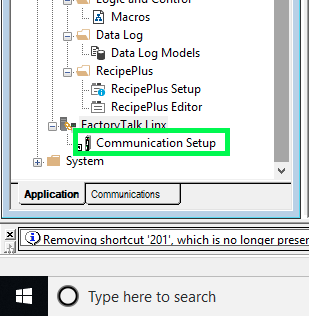
\includegraphics[width=3.2in]{CommunicationSetup}}
\caption{Where to find the HMI Communication Setup}
\label{fig:HMICommunicationSetup}
\end{figure}

In the window that opens, navigate to the PLC associated with your lab seat. \textbf{Click the plus beside the PLC associated with your lab seat}. \textbf{Click the plus beside the item named PointBus}. Now, \textbf{highlight the item 0}. Refer to \figureautorefname \ref{fig:PLCSelectionHMISetup} for clarification.

\aside{In \figureautorefname \ref{fig:PLCSelectionHMISetup} the user was sitting in seat number 1. \textbf{You most likely will not select the same PLC IP address shown in the image.} Refer to \tableautorefname \ref{Table:PLCIpAddresses} to verify which IP address is associated with your seat.}

\begin{figure}[h]
\centering
\textbf{Select the PLC in the HMI Software}\par \medskip
\frame{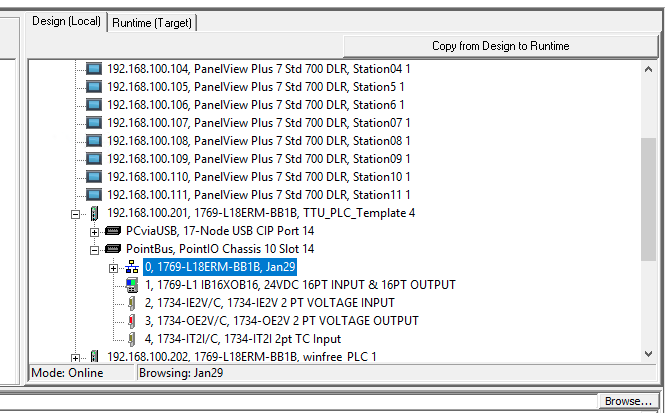
\includegraphics[width=3.2in]{SelectPLCinHMI}}
\caption{PLC Selection in HMI Communication Setup}
\label{fig:PLCSelectionHMISetup}
\end{figure}

With the correct PLC highlighted, \textbf{highlight PLC in the Device shortcuts to the left and click apply}. Next, \textbf{click copy from design to runtime}. Refer to \figureautorefname \ref{fig:CopyfromDesignToRuntime} to clarify.

\begin{figure}[h]
\centering
\textbf{Copy from design to runtime}\par \medskip
\frame{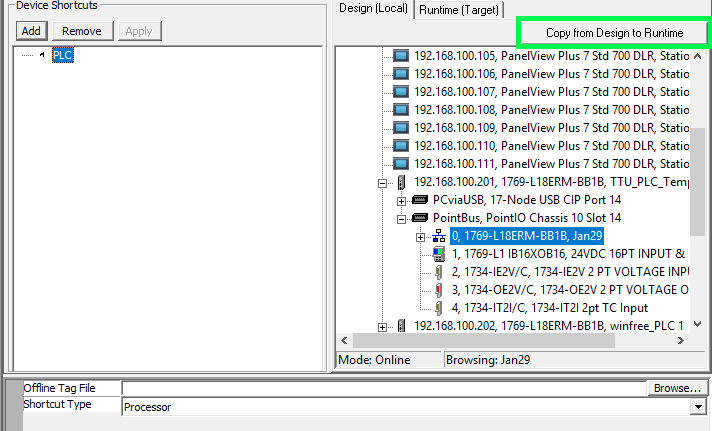
\includegraphics[width=3.2in]{CopyFromDesignToRuntime}}
\caption{Location of copy from design to runtime button}
\label{fig:CopyfromDesignToRuntime}
\end{figure}

The last step to setting up the communication between the PLC and HMI is to accept the communication settings that you have now put in place. To do this click OK in the lower right of the window. Refer to \figureautorefname \ref{fig:FinalizeCommunicationSettings}.

\begin{figure}[h]
\centering
\textbf{Finalize communication setup}\par \medskip
\frame{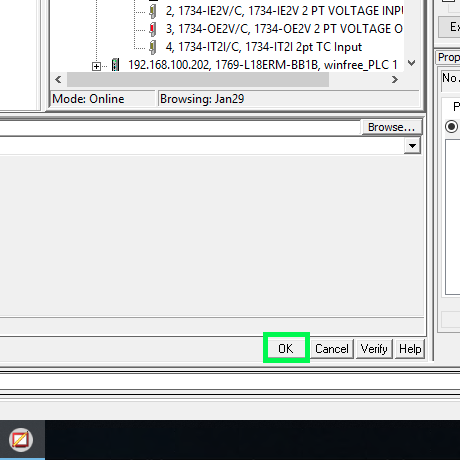
\includegraphics[width=3.2in]{FinalizeCommunicationSettings}}
\caption{Ok to finalize HMI/PLC communication setup}
\label{fig:FinalizeCommunicationSettings}
\end{figure}


\subsection{Create the Runtime Application}

Go to the Application menu and select \textbf{Create Runtime Application}. In the dialog window that appears, \textbf{select save}. This compiles the application into an HMI "runtime". A "Runtime" is what is downloadable to the HMI. 

\subsection{Download the HMI application}

Go to the tools menu and select \textbf{Transfer Utility}. This opens another application which is used to transfer the HMI runtime application to the physical HMI. In the window that appears do the following:

\begin{enumerate}
    \item Click the box with the ellipse next to the source file entry bar
    \item Select the application you created and click open
    \item Check the box beside \textbf{run application at startup}
    \item Check the box beside \textbf{replace communications when transferring the HMI application}
\end{enumerate}

Next you must select the IP address associated with the HMI to which you would like to download the runtime application. The HMI IP address is also associated with your lab seat. Refer to \tableautorefname \ref{Table:HMIIpAddresses} to find the IP address of the HMI associated with your lab seat. 

After identifying the correct HMI IP address, \textbf{highlight the appropriate HMI in the transfer utility window and select download}.

\aside{You may be prompted that an application with this name already exists in the HMI. It is ok to overwrite the existing application.}

\begin{table}[h]
\centering
\caption{HMI IP addresses}
\label{Table:HMIIpAddresses}
\begin{tabular}{c l | c l}
\toprule
Seat \# & IP Address & Seat \# & IP Address\\
\midrule
1 & $192.168.100.101$ & 2 & $192.168.100.102$ \\
3 & $192.168.100.103$ & 4 & $192.168.100.104$ \\
5 & $192.168.100.105$ & 6 & $192.168.100.106$ \\
7 & $192.168.100.107$ & 8 & $192.168.100.108$ \\
9 & $192.168.100.109$ & 10 & $192.168.100.110$ \\
11 & $192.168.100.111$ & 12 & $192.168.100.112$ \\
\bottomrule
\end{tabular}
\end{table}

\subsection{Testing the HMI application}

Once the download completes and the HMI reboots, the application should be running on the HMI screen. There should be a button and display. 

The button has the text "check code". This will check to see if the edits you make to the code in the coming sections is correct. If it is correct, the HMI will tell you that you have correctly written the code. If you hold down the button it will display the word release, instructing you to stop pressing the button.

\aside{For the first several labs we will provide an HMI application that you must download to the HMI. The HMI application will work with code built into the lab PLC file that we provide to notify you if your code is correct and give you feedback.}

\TASignatureSlot


\section{Online ladder program edits}

There are two ways to edit the PLC program. The first is called an online edit and the second is an offline program edit. Online program edits allow the programmer to change the code while the PLC is still in Run mode. An offline PLC program edit requires a download after the edit is complete. Anytime a programmer downloads to the PLC, the PLC is automatically taken out of Run mode and put into Program mode. Typically, after the download completes the programmer is prompted to put the PLC back into Run mode.

\aside{In a laboratory environment it is fine to stop the PLC from executing briefly to perform a download. However, imagine what would happen if the PLC that is used to control the Tennessee Tornado at DollyWood were to be taken out of Run mode in the middle of a ride!}

In this section you will be making an online edit to the program to fix the logical error in the lab 0 program.

\subsection{What's wrong with the logic}

Before you can edit the program, you must figure out what is wrong with the logic. In \figureautorefname \ref{fig:TheCode}, the code is shown. The code is intended to decide if it is Fall based on the month. This doesn't mean that it is deciding if it is Fall based on the current month in the real world, but rather based on which month is "on". 

The add on instruction (AOI) in the upper right hand corner of  \figureautorefname \ref{fig:TheCode} called Lab0\textunderscore IsItFallYet has several attributes associated with it. Some are inputs and some are outputs. Particularly, it has the attributes shown in \tableautorefname \ref{Table:Lab0.1Attributes}.

To access any of these attributes, the dot operator is used. This is why above the contact on the left side of the rung of code in \figureautorefname \ref{fig:TheCode} it says "Lab0.October". Lab0 is the name given to the \textbf{tag} that houses all the memory for the Lab0\textunderscore IsItFallYet
AOI.

\aside{An AOI (add on instruction) is an instruction that someone other than Allen Bradley has created. The AOI requires memory. The way that Allen Bradley allocates memory is in the form of tags. So, there must be a tag associated with each occurrence of an AOI in the code.}

So, if the "Lab0.October" bit (boolean tag) is true (or on, or energized) that would mean that it is October. If the "Lab0.October" bit is on then the normally open contact it is associated with will be energized. Think of this like a light switch. If the "Lab0.October" light switch is on, then electricity will pass through it. 

Keeping with the electrical analogy, now that the switch (referred to as a contact) associated with "Lab0.October" is on (because "Lab0.October" is on), then the voltage on the left hand side of the ladder will pass through to the right hand side of the contact associated with "Lab0.October". This voltage will continue along the rung and be applied to the coil associated with the attribute "Lab0.Its\textunderscore Fall". Energizing the a coil associated with a boolean tag sets the value of the tag to true. \textbf{So, if "Lab0.October" is on, then "Lab0.Its\textunderscore Fall" is also on}.

\aside{The left hand side of an instruction (like the normally open contact associated with "Lab0.October") is called the \rungincondition. The right hand side of an instruction is called the \rungoutcondition. If a normally open contact is on (the boolean value associated with the contact is true), then the \rungoutcondition is set equal to the \rungincondition. However, if the normally open contact is off (the boolean value associated with the contact is false), then the \rungoutcondition is always set to off (or low voltage).}

What about if "Lab0.November" is on but "Lab0.October" is off? The \rungoutcondition for the "Lab0.October" contact is off. However, the \rungincondition applied to the "Lab0.November" is on so the \rungoutcondition is also on. So, a high voltage is still applied to the "Lab0.Its\textunderscore Fall" coil.

\begin{table}[h]
\centering
\caption{Attributes available in Lab0}
\label{Table:Lab0.1Attributes}
\begin{tabular}{c c c}
\toprule
Attribute Name & Data Type & Type\\
\midrule
Jan & Bool & Output \\
Feb &  Bool & Output \\
March &  Bool & Output \\
April & Bool & Output \\
May &  Bool & Output \\
June &  Bool & Output\\
July &  Bool & Output \\
August &  Bool & Output \\
September &  Bool & Output \\
October &  Bool & Output \\
November &  Bool & Output \\
December &  Bool & Output \\
\midrule
Its\textunderscore Fall & Bool & Input\\
\bottomrule
\end{tabular}
\end{table}

\subsubsection{What does the code mean logically}

This rung of code implements a logical OR. If either "Lab0.October" OR "Lab0.November" is true, then "Lab0.Its\textunderscore Fall" is also true. If both "Lab0.October" AND "Lab0.November" are false, then "Lab0.Its\textunderscore Fall" is false.

\subsubsection{What should it be?}

In reality, October and November aren't the only Fall months. September is also a Fall month. So, we need to modify the logic so that if either "Lab0.October" OR "Lab0.November" OR "Lab0.September" is true then "Lab0.Its\textunderscore Fall" is also true. 

\subsection{Let's fix this code}

Now that we have identified the problem with the present code, it is time to fix the problem. To do so we are going to make an online edit to the program.

\subsubsection{Making the rung editable}

To edit a rung of code while the programmer (you) is online, \textbf{right click on the number to the left of the rung and select "Start pending rung edits"}. Two versions of the rung will then be on the screen. The top version will have a column of small letter i's to the left of the rung while the bottom has a column of small letter r's to the left of the rung.

\subsubsection{Adding another OR condition}

We want to add another path for the voltage to flow in the case where "Lab0.September" is true. To do this we must first modify the structure of the rung and then add the instructions.

To modify the structure of the rung, highlight the left side of the rung beside "Lab0.November". This is shown in \figureautorefname \ref{fig:HighlightRung}. The next step, shown in \figureautorefname \ref{fig:AddBranch}, is to add a branch to the rung structure. After the branch is added, it needs to be adjusted to suit our needs. Click and drag the right side of the branch so that it matches what is shown in \figureautorefname \ref{fig:DragTheBranch}.

\begin{figure}[h]
\centering
\textbf{Highlight the rung}\par \medskip
\frame{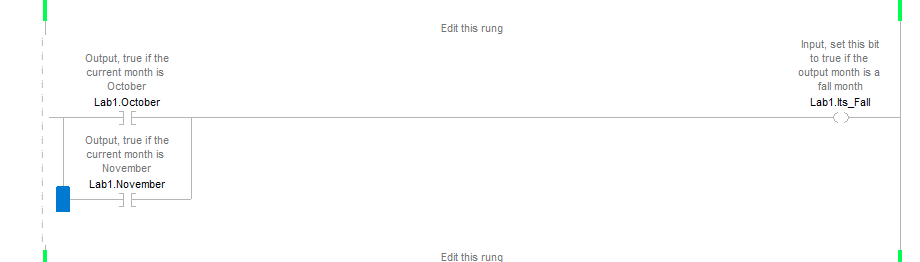
\includegraphics[width=3.2in]{HighlightRung}}
\caption{Highlight the rung that is going to be structurally modified}
\label{fig:HighlightRung}
\end{figure}


\begin{figure}[h]
\centering
\textbf{Add a branch}\par \medskip
\frame{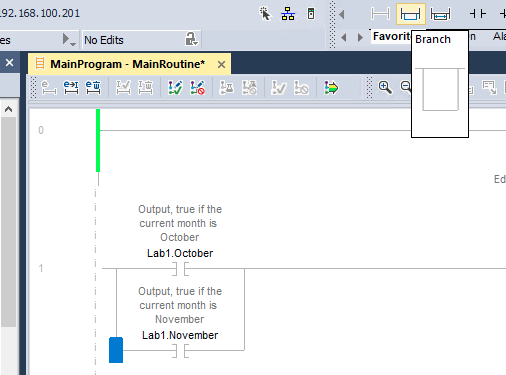
\includegraphics[width=3.2in]{AddBranch}}
\caption{Add a branch to the rung structure}
\label{fig:AddBranch}
\end{figure}


\begin{figure}[h]
\centering
\textbf{Click and drag the branch}\par \medskip
\frame{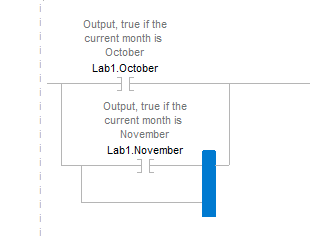
\includegraphics[width=3.2in]{DragTheBranch}}
\caption{Click and drag the branch to suit your needs}
\label{fig:DragTheBranch}
\end{figure}


After the rung is structurally changed to suit our purposes, you must add a contact to adjust the rung logic. Highlight the left hand side of the newly created branch and insert a normally open contact. Refer to \figureautorefname \ref{fig:AddContact}.

\begin{figure}[h]
\centering
\textbf{Add a contact to the branch}\par \medskip
\frame{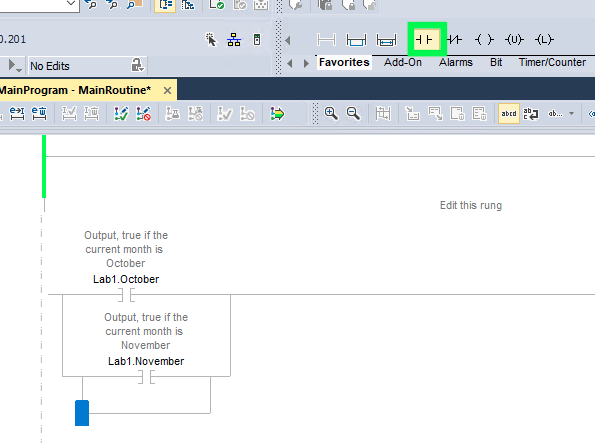
\includegraphics[width=3.2in]{AddContact}}
\caption{Add a contact to the branch}
\label{fig:AddContact}
\end{figure}

At this point there is no tag associated with the contact instruction. So, a question mark appears above the contact. To complete the changes we need to associate this new contact with "Lab0.September". To do this, select the question mark above the contact and type "Lab0.September" without the quotation marks. Press enter when it is fully typed.

\subsubsection{Submitting online edits}

The last step to completing our online edit is to finalize all the edits in the program. To finalize the edits click the button shown in \figureautorefname \ref{fig:FinalizeEdits}. A dialog window will appear asking you to confirm that you wish to finalize the edits. Select yes. If your code did not have any errors, then the code is finalized and is now running in the PLC.

\begin{figure}[h]
\centering
\textbf{Finalize all edits in program}\par \medskip
\frame{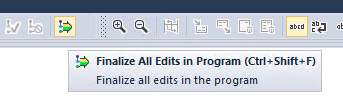
\includegraphics[width=3.2in]{FinalizeEdits}}
\caption{Finalize the online program edits}
\label{fig:FinalizeEdits}
\end{figure}

\subsection{Is it Fall yet?}

Now, press the check code button on the HMI. If you edited the code correctly then your HMI will say so. 

\TASignatureSlot


\section{Offline ladder program edits}

Another way to edit the code, as stated previously, is to take the program offline. While the code is offline, all rungs (in general) are editable. This is often convenient if you have several rungs to edit. However, you will have to perform a download after making offline changes to a program.

In this section you will make an offline edit to the program and download the edited code.

\subsection{How do you know that it is Fall?}

First, let's consider a logical question. How does one know that it is Fall based on the month? Certainly we have found one answer to this question. But is there another way? 

The solution we have used thus far is to check if it is October OR November OR September. If any of these is true then it is also true that it is Fall.

Instead of using a logical OR we can also use the logical AND to infer the state of Fall. The logic goes like this: if it is \textit{not} January AND \textit{not} February AND \textit{not} March AND \textit{not} April AND \textit{not} May AND \textit{not} June AND \textit{not} July AND \textit{not} August AND \textit{not} December, then it must be Fall. 

\subsection{Let's code it}

In order to write this into code, you will have to make use of the normally closed contact (XIO). The normally closed contact will allow the voltage to pass if the boolean tag associated with the normally closed contact is false. This allows us to code \textit{not} January and so forth.

Structurally, the conditions won't be in branches that pass around each other. Rather, each of the normally closed contacts will be placed in series so that the only way for voltage to get to the coil associated with "Lab0.Its\textunderscore Fall" is for the boolean attributes associated with all non-Fall months to be false.

\aside{If a normally closed contact is on (the boolean value associated with the contact is true), then the \rungoutcondition is set to false. However, if the normally closed contact is off (the boolean value associated with the contact is false), then the \rungoutcondition is always set equal to the \rungincondition.}

\aside{XIO and XIC are the actual names of the Allen Bradley normally closed and normally open contacts respectively. The acronym stands for "examine if open" and "examine if closed".\\
--Normally closed means that the normal (not energized) state is closed. This would be like a light switch that allowed current to flow when it was off but stopped the flow of current when the switch was in the on position (a backwards light switch). This is the same as "examine if open".\\
--Normally open means that the normal (not energized) state is open. This would be like a light switch that allowed current to flow when it was on but stopped the flow of current when the switch was in the off position (a typical light switch). This is the same as "examine if closed".}

\subsubsection{Go Offline}

To set the PLC to offline, \textbf{select go offline} under the communications menu.

\subsubsection{Edit the rung - Delete the conditions}

Edit the rung appropriately so that it looks like the one shown in \figureautorefname \ref{fig:NotLogic}.


\begin{figure}[h]
\centering
\textbf{AND based logical approach}\par \medskip
\frame{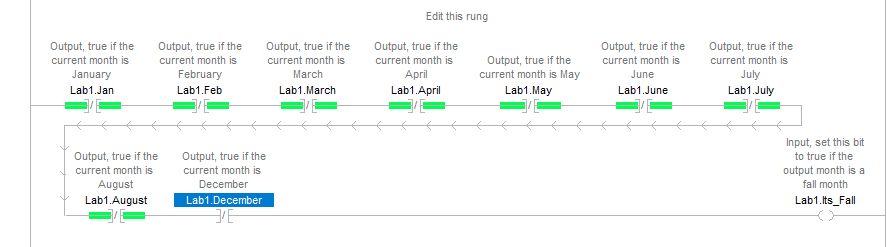
\includegraphics[width=3.2in]{NotLogic}}
\caption{AND based logical approach to deciding it is Fall}
\label{fig:NotLogic}
\end{figure}

\subsubsection{Download}

Download the code to the PLC. If you need guidance on the process, refer to \sectionautorefname \ref{subsection:DownloadPLC}.

\subsubsection{Go Online}

Go online. If you need guidance on the process, refer to \sectionautorefname \ref{subsection:GoOnline}.

\subsection{Is it Fall yet?}

Again press the button on the HMI. If your new logic is correct then HMI will display the same message you saw previously when you fixed the logic used to decide if it is Fall.

\TASignatureSlot


\section{Toggle a bit}

Sometimes it is helpful to be able to toggle a bit from off (false) to on (true) as well as vice versa. Specifically, this is helpful when you want to test a logical circuit under certain conditions.

\subsection{Toggle December}

Allen Bradley provides a convenient keyboard shortcut to toggle a bit. To demonstrate this, highlight the normally closed contact associated with "Lab0.December". With it highlighted, hold the control key and press the T key (ctrl+T). This will change the boolean value of "Lab0.December".

Now, highlight the coil associated with "Lab0.Its\textunderscore Fall" and use the toggle keyboard shortcut.

Why do you think that it doesn't appear to work?

\aside{The PLC is executing the code continuously while in Run mode. This execution happens in under a few milliseconds on an Allen Bradley PLC. So, if you attempt to toggle the state of a boolean tag which is being "driven" (another term for being associated with a coil), then the PLC quickly overwrites the result of your toggle command with the logical result from the output coil.}

Demonstrate your ability to use the toggle shortcut to the TA.

\TASignatureSlot
\chapter{Pre-Lab 1}
\setcounter{TASignatures}{0}
\setcounter{AsideCounter}{0}


\section{Introduction}

Make sure to complete this pre-lab before your assigned lab time. You will not be allowed to begin working on your lab without having this complete.



Each of the following problems are to be completed on paper. You are not expected to program these problems on PLC. You are expected to write neat ladder logic diagrams on paper.



\section{Problem 1}

Convert the code shown in \figureautorefname \ref{fig:Problem1} to a rung of ladder logic.

\lstset{style=mystyle}
\lstset{language=python}
\begin{figure}[h]
\begin{lstlisting}[firstnumber=1]

while(True){
    if(Pallet_Present and not Station_In_Operation):
        Sound_Alarm = True
    else:
        Sound_Alarm = False
}
    
\end{lstlisting}
\caption{Pre-lab problem 1}
\label{fig:Problem1}
\end{figure}


\section{Problem 2}

Convert the code shown in \figureautorefname \ref{fig:Problem2} to a rung of ladder logic.

\lstset{style=mystyle}
\lstset{language=python}
\begin{figure}[h]
\begin{lstlisting}[firstnumber=1]

while(True){
    if(not Robot_Home and 
        (Door_Open or Person_In_Guard)):
        E_Stop = True
    else:
        E_Stop = False
}
    
\end{lstlisting}
\caption{Pre-lab problem 2}
\label{fig:Problem2}
\end{figure}


\section{Problem 3}

Convert the code shown in \figureautorefname \ref{fig:Problem3} to a rung of ladder logic.

\lstset{style=mystyle}
\lstset{language=python}
\begin{figure}[h]
\begin{lstlisting}[firstnumber=1]

while(True){
    if(Station1_Home and Station2_Home
        and (Station3_Home and Station4_Home
        and (Station5_Home or Station6_Home))
        or Bypassed):
        Safe_To_Move = True
    else:
        Safe_To_Move = False
}
    
\end{lstlisting}
\caption{Pre-lab problem 3}
\label{fig:Problem3}
\end{figure}

\section{Problem 4}

In electrical engineering, the $+$ operator signifies a logical OR operation. The $\cdot$ operator is used to signify the logical AND operation. Lastly, the bar over top of an element(s) signifies the logical NOT operation.

So, the boolean formula shown in \equationautorefname \ref{equ:lab} is functionally equivalent to the sequential logic shown in \figureautorefname \ref{fig:Problem4}.

\begin{align}
    \label{equ:lab}
    D = \overline{((A+B)\cdot C\cdot A)}
\end{align}


\lstset{style=mystyle}
\lstset{language=python}
\begin{figure}[h]
\begin{lstlisting}[firstnumber=1]

while(True){
    if(not ((A or B) and C and A)):
        D = True
    else:
        D = False
}
    
\end{lstlisting}
\caption{Pre-lab problem 4}
\label{fig:Problem4}
\end{figure}

Programming this in a single rung of ladder logic in a PLC would be a bit difficult however, because the entire formula is negated. So, we need a way to transform the formula so that the formula is not negated.  

DeMorgan's theorem states the following property for boolean formulae:
\begin{align}
\overline{(A\cdot B)} =& \overline A + \overline B \\
\overline{(A + B)} =& \overline A\cdot \overline B
\end{align}

Apply DeMorgan's theorem to transform \equationautorefname \ref{equ:lab} into a more ladder logic friendly format. 

Using your transformed version of the formula, write the appropriate \textbf{single rung} of ladder logic to assign the tag $D$ the value true if \equationautorefname \ref{equ:lab} is true. Else, $D$ should be assigned the value false.

\aside{To help you solve this, here is an example of DeMorgan's law used to transform a boolean formula. 
\begin{align*}
U &= \overline{(X\cdot (Y + Z))}  && \text{Original formula}\\  
&= \overline X + \overline{(Y + Z)} && \text{DeMorgan's applied to outer parenth}\\
&= \overline X + (\overline Y \cdot \overline Z)&& \text{DeMorgan's applied to inner parenth}
\end{align*}
}

\section{Problem 5 - Read the Manual}

Read the lab manual. Then write a paragraph about the content and expectations in the lab manual which will convince the grader that you have in fact read the complete lab manual.

\chapter{Lab 1}
\setcounter{TASignatures}{0}
\setcounter{AsideCounter}{0}

\section{Introduction}
    \vspace{0.1em}

    \textbf{In this lab you gain experience with:}
    \begin{enumerate}
        \item Analyzing how a ladder logic program will execute
        \item Using the output coil (OTE)
        \item Using the normally closed contact (XIO)
        \item Using the normally open contact (XIC)
        \item Coding various logical problems
    \end{enumerate}

\subsection{Lab Files}

Go to iLearn and download the PLC and HMI files for this lab to the PC. Then download the PLC project to the PLC and the HMI application to the HMI. 

\subsection{Acceptable Instructions}

You may have previous experience with PLCs and that is great! However, you are only allowed to use the instructions that we have covered thus far in the lab. So, if you have experience already, consider it a challenge to restrict yourself to only use the instructions that have been covered thus far in lecture to solve the problem!

\subsection{How to Interface with the PLC and HMI}
\begin{samepage}
\noindent If you are unclear on any of the following, refer to the Lab 1 Manual:
\begin{enumerate}
    \item Download to the PLC
    \item Go online with the PLC
    \item Put the PLC into Run Mode
    \item Make online and offline edits to the PLC program
    \item Download to the HMI
    \item Toggle a boolean tag
\end{enumerate}

\end{samepage}

\subsection{How to get credit}
Each lab after this will require each student to submit the completed pre-lab before they are allowed to begin working on the lab. The \textbf{pre-lab must be submitted to the TA before beginning work on the lab}. If it is not complete then you will be required to complete the pre-lab before you are allowed to begin working on the lab.

In order to get credit for completing each part of this lab, \textbf{you must personally read and complete each portion of the lab and demonstrate the completion to the TA}. Each section has one or more signature slots that must be signed by the TA to confirm that the section was completed. Each section is worth equal credit. 

\subsection{20 minute grace period}
To receive full credit, the lab must be completed and demonstrated during the assigned lab time. However, if you cannot complete the lab within that time, you can complete and demonstrate the lab within the first 20 minutes of the subsequent lab time and still receive full credit. \textbf{If the lab is not completed within the assigned lab time and is not completed within the 20 minute grace period, then the lab is considered late}. If you submit the lab late, then there will be a 20\% deduction compounded weekly.


\subsection{Lab agreement}

The planning of a program is often a very social activity, however the actual writing of the code is always an individual pursuit. In this class it is very much the same. Students are welcome to verbally assist each other, but each person is required to write their own code and personally complete each lab. In this way each student will gain valuable experience with programming PLCs. 

\textbf{The undersigned person guarantees that any and all work demonstrated to the TA in regard to this lab is a result of their own work with no unauthorized help.}

\signatureSlot{Student (Print \& Sign)}


\section{Storefront Door Controller}

This section corresponds to the \verb|Lab1_1| object in the Lab1 PLC file.
\\ 
\\
Picture it, you have just graduated and a local grocery store contacts you and asks if you would be willing to do some freelance engineering/programming work for them. The first thing they ask you to do is to make their automatic doors work. They hired a company to install the automatic door system but the contract was disputed and the company left the work unfinished.

When you arrive at the store you find that the motor that opens the door is connected to an Allen Bradley PLC! You also find that the sensor used to detect the presence of a person in front of the door is also connected to the PLC. The PLC also gets a signal from the security system to know that the store is open for business. So, all that's left for you to do is program the PLC to control the signal that goes to the door.

\subsection{How should the logic work?}

Simple. Any time the store is open and someone is detected in front of the doors, then the doors should open.

This logic in normal sequential programming would look something like that shown in \figureautorefname \ref{fig:2_1Sequential}

\lstset{style=mystyle}
\lstset{language=python}
\begin{figure}[h]
\begin{lstlisting}[firstnumber=1]
if (Lab1_1.Store_Is_Open and
        Lab1_1.Person_Present_At_Front_Of_Door):
    Lab1_1.Open_The_Door = True
else:
    Lab1_1.Open_The_Door = False
\end{lstlisting}
\caption{Sequential logic similar to Lab1 part 1}
\label{fig:2_1Sequential}
\end{figure}

\subsection{The Inputs and Outputs}

To access any of the signals listed in \tableautorefname \ref{Table:Lab1_1Attributes}, use the syntax \verb|Lab1_1.| followed by the attribute name. 

\begin{table}[h]
\centering
\caption{Attributes available in Lab1\textunderscore 1}
\label{Table:Lab1_1Attributes}
\begin{tabular}{c c c}
\toprule
Attribute Name & Data Type & Type\\
\midrule
\verb|Store_Is_Open| & Bool & Output \\
\verb|Person_Present_At_Front_Of_Door| &  Bool & Output \\
\midrule
\verb|Open_The_Door| & Bool & Input\\
\bottomrule
\end{tabular}
\end{table}

Write the appropriate logic in the associated rung in the PLC file.

\TASignatureSlot



\section{Storefront Door Controller... again}

This section corresponds to the \verb|Lab1_2| object in the Lab1 PLC file.
\\ 
\\
When you left the grocery store, the door worked beautifully and your customer was very happy. However, after a few hours you receive a frantic phone call from the store manager asking you to return to the store because there was a problem with the doors!

When you return to the store you find that the store is packed with people but they are all standing inside looking out the front door like a hoard of zombies! What could cause such a weird situation? Well, it seems that your door programming works well at letting people in but since the sensor used to detect people at the back of the door was never connected you did not think to add it. So, people can get in but no one can get out because the \verb|Person_Present_At_Front_Of_Door| signal doesn't work for people at the back of the door.

\aside{The first automatic doors were designed by Heron of Alexandria in the first century AD! He made a mechanism driven by the heat from a fire that was kindled by priests in the temple to cause a water counter balance to open the temple door.}

You quickly install the motion detection sensor used to detect the presence of a person at the back of the door and connect the sensor to the PLC. Now you have to rewrite your code!

\subsection{How should the logic work?}

If the store is open and a person is in front of the doors or in back of the doors, then the doors should be open.

This logic in normal sequential programming would look something like that shown in \figureautorefname \ref{fig:2_2Sequential}

\lstset{style=mystyle}
\lstset{language=python}
\begin{figure}[h]
\begin{lstlisting}[firstnumber=1]

if (Lab1_2.Store_Is_Open and
        (Lab1_2.Person_Present_At_Front_Of_Door or
        Lab1_2.Person_Present_At_Back_Of_Door)):
    Lab1_2.Open_The_Door = True
else:
    Lab1_2.Open_The_Door = False
    
\end{lstlisting}
\caption{Sequential logic similar to Lab1 part 2}
\label{fig:2_2Sequential}
\end{figure}

\subsection{The Inputs and Outputs}

To access any of the signals listed in \tableautorefname \ref{Table:Lab1_2Attributes}, use the syntax \verb|Lab1_2.| followed by the attribute name. 

\begin{table}[h]
\centering
\caption{Attributes available in Lab1\textunderscore 2}
\label{Table:Lab1_2Attributes}
\begin{tabular}{c c c}
\toprule
Attribute Name & Data Type & Type\\
\midrule
\verb|Store_Is_Open| & Bool & Output \\
\verb|Person_Present_At_Front_Of_Door| &  Bool & Output \\
\verb|Person_Present_At_Back_Of_Door| &  Bool & Output \\
\midrule
\verb|Open_The_Door| & Bool & Input\\
\bottomrule
\end{tabular}
\end{table}

Write the appropriate logic in the associated rung in the PLC file.

\TASignatureSlot


\section{Sawmill controller}

This section corresponds to the \verb|Lab1_3| object in the Lab1 PLC file.
\\ 
\\

Word got out that you were a good programmer (even with the minor blunder with the zombie hoard at the grocery store). Pretty soon you are contacted by the owner of a sawmill that wants to replace the old relay system that currently controls the saw with a PLC based system.



\subsection{How should the logic work?}

The current system requires the saw operator press the start button to start the saw. But once the saw is running, it will remain running until the stop button is pressed. He wants the saw to work precisely the same way after you are done. 

\aside{What the sawmill owner wants is referred to in ladder logic as a \textbf{seal-in}. It is a useful way of keeping a coil energized (on) once it has been turned on. This is a very important concept in PLC programming.}

This logic in normal sequential programming would look something like that shown in \figureautorefname \ref{fig:2_3Sequential}

\lstset{style=mystyle}
\lstset{language=python}
\begin{figure}[h]
\begin{lstlisting}[firstnumber=1]

if ((Lab1_3.Start_Saw or Lab1_3.Run_Saw) and 
        not Lab1_3.Stop_Saw):
    Lab1_3.Run_Saw = True
else:
    Lab1_3.Run_Saw = False
    
\end{lstlisting}
\caption{Sequential logic similar to Lab1 part 3}
\label{fig:2_3Sequential}
\end{figure}

\subsection{The Inputs and Outputs}

To access any of the signals listed in \tableautorefname \ref{Table:Lab1_3Attributes}, use the syntax \verb|Lab1_3.| followed by the attribute name. 

\begin{table}[h]
\centering
\caption{Attributes available in Lab1\textunderscore 3}
\label{Table:Lab1_3Attributes}
\begin{tabular}{c c c}
\toprule
Attribute Name & Data Type & Type\\
\midrule
\verb|Start_Saw| & Bool & Output \\
\verb|Stop_Saw| &  Bool & Output \\
\midrule
\verb|Run_Saw| & Bool & Input\\
\bottomrule
\end{tabular}
\end{table}

Write the appropriate logic in the associated rung in the PLC file.

\TASignatureSlot



\section{Challenge}

This section corresponds to the \verb|Lab1_4| object in the Lab1 PLC file.
\\ 
\\

You decided that to get more publicity you would enter a PLC programming competition that sends out challenges once a week. If you win there's even a guaranteed job offer! This week the contest judges decided that each competitor must code a boolean formula into a single rung of ladder logic using only the normally closed contact, normally open contact, and the coil instructions. The formula that they have given is $D = \overline{((A+B)\cdot C\cdot A)}$. 

The reason that this is challenging is because there is no good way to negate a group of logical operations in ladder logic in a single rung. The key is to use Demorgan's theorem to transform the boolean formula into one that \textbf{doesn't have any logical NOT operations applied to a group}. 

\aside{In electrical engineering, the $+$ operator signifies a logical OR operation. The $\cdot$ operator is used to signify the logical AND operation. Lastly, the bar over top of an element(s) signifies the logical NOT operation.}

\aside{Demorgan's theorem states that:
\begin{align}
\overline{(A\cdot B)} =& \overline A + \overline B \\
\overline{(A + B)} =& \overline A\cdot \overline B
\end{align}}

\aside{This situation comes up often in industrial PLC applications. Before a robot is allowed to interface with a sub-section of a machine, the machine must be at rest (otherwise you risk damaging the machine). This typically involves making sure that a group of things are NOT true. Negating the group is ugly in ladder logic and it is typically better to apply Demorgan's theorem to get the boolean formula into a more manageable form.}

\subsection{How should the logic work?}

That's for you to figure out!

\subsection{The Inputs and Outputs}

To access any of the signals listed in \tableautorefname \ref{Table:Lab1_4Attributes}, use the syntax \verb|Lab1_4.| followed by the attribute name. 

\begin{table}[h]
\centering
\caption{Attributes available in Lab1\textunderscore 4}
\label{Table:Lab1_4Attributes}
\begin{tabular}{c c c}
\toprule
Attribute Name & Data Type & Type\\
\midrule
\verb|A| & Bool & Output \\
\verb|B| &  Bool & Output \\
\verb|C| &  Bool & Output \\
\midrule
\verb|D| & Bool & Input\\
\bottomrule
\end{tabular}
\end{table}

\TASignatureSlot
\input{Labs/PreLab2}
\chapter{Lab 2}
\setcounter{TASignatures}{0}
\setcounter{AsideCounter}{0}

\section{Introduction}
    \vspace{0.1em}

    \textbf{In this lab you gain experience with:}
    \begin{enumerate}
        \item Analyzing how a multi-rung ladder logic program will execute
        \item Using the output Latch (OTL)
        \item Using the output Unlatch (OTU)
        \item Storing the result of a rung in a tag
        \item Accomplishing logical functionality using on a multi-scan approach
    \end{enumerate}

\subsection{Lab Files}

Go to iLearn and download the PLC and HMI files for this lab to the PC. Then download the PLC project to the PLC and the HMI application to the HMI. 

\subsection{Acceptable Instructions}

You may have previous experience with PLCs and that is great! However, you are only allowed to use the instructions that we have covered thus far in the lab. So, if you have experience already, consider it a challenge to restrict yourself to only use the instructions that have been covered thus far in lecture to solve the problem!

\subsection{How to Interface with the PLC and HMI}
\begin{samepage}
\noindent If you are unclear on any of the following, refer to the Lab 1 Manual:
\begin{enumerate}
    \item Download to the PLC
    \item Go online with the PLC
    \item Put the PLC into Run Mode
    \item Make online and offline edits to the PLC program
    \item Download to the HMI
    \item Toggle a boolean tag
\end{enumerate}

\end{samepage}

\subsection{How to get credit}
The \textbf{pre-lab must be submitted to the TA before beginning work on the lab}. If it is not complete then you will be required to complete the pre-lab before you are allowed to begin working on the lab.

In order to get credit for completing each part of this lab, \textbf{you must personally read and complete each portion of the lab and demonstrate the completion to the TA}. Each section has one or more signature slots that must be signed by the TA to confirm that the section was completed. Each section is worth equal credit. 

\subsection{20 minute grace period}
To receive full credit, the lab must be completed and demonstrated during the assigned lab time. However, if you cannot complete the lab within that time, you can complete and demonstrate the lab within the first 20 minutes of the subsequent lab time and still receive full credit. \textbf{If the lab is not completed within the assigned lab time and is not completed within the 20 minute grace period, then the lab is considered late}. If you submit the lab late, then there will be a 20\% deduction compounded weekly.


\subsection{Lab agreement}

The planning of a program is often a very social activity, however the actual writing of the code is always an individual pursuit. In this class it is very much the same. Students are welcome to verbally assist each other, but each person is required to write their own code and personally complete each lab. In this way each student will gain valuable experience with programming PLCs. 

\textbf{The undersigned person guarantees that any and all work demonstrated to the TA in regard to this lab is a result of their own work with no unauthorized help.}

\signatureSlot{Student (Print \& Sign)}



\section{Box Transfer System}

This section corresponds to the \verb|Lab2_1| object in the Lab2 PLC file. \textbf{You will have to create tags to be able to build a bit latch sequence as demonstrated in lecture}.
\\ 
\\

Congratulations are in order. You have just landed a big contract with a certain online retailer that ships thousands of packages a day (you know the one). They have a heavy parcel moving machine that they use to transfer heavy packages from their conveyor to the truck. However, at the moment the machine must be controlled by a human operator. The online retailer has tasked you with automating the task. 


\subsection{How should the logic work?}


They want you to write a ladder logic program that will be initiated by a button connected to a signal in the PLC called \verb|Start_Transfer|. When \verb|Start_Transfer| is pressed, the parcel mover will go vertically up until it reaches a switch called \verb|Transfer_Raised|. Then it will move horizontally until it reaches the switch called \verb|Transfer_Extended|. Then the transfer will lower until it reaches the \verb|Transfer_Lowered| switch. 

\aside{Machines like this heavy parcel transfer system are typically pneumatically driven. Each of the motions made possible by a pneumatic cylinder. Each of the cylinders is connected to pneumatic valves which are controlled by the PLC. Pneumatic cylinder control is the most common way to implement motion in factories today!}

In order to tell the heavy parcel transfer machine to raise, extend, and lower use the \verb|Raise_Transfer|, \verb|Extend_Transfer|, and \verb|Lower_Transfer| signals respectively. The transfer movement doesn't happen immediately. Rather, you must hold the command for a full second before the action takes place. Play with the associated HMI display to get an idea of how the transfer movement happens. When you program this to take place automatically, the command to take an action should be held until the feedback signal becomes true. ie. if \verb|Raise_Transfer| is true for more than 1000 milliseconds then \verb|Transfer_Raised| should change to true.

Hint: Make sure that you turn off \verb|Raise_Transfer| before turning on \verb|Lower_Transfer| or nothing will happen. This is also be true with \verb|Extend_Transfer| and \verb|Retract_Transfer|, but there is no need in this lab to use the \verb|Retract_Transfer| signal.

Hint: You will need to create bits to make a bit latch sequence like the one discussed in the lecture.

\aside{If you energize both sides of a double-acting cylinder (a pneumatic cylinder that can be extended and retracted) with air, it will remain stationary.}

\subsection{The Inputs and Outputs}

Once you have programmed the bit latch sequence to control the parcel machine, you should be able to press the start transfer button on the HMI and see the parcel move to the truck.

To access any of the signals listed in \tableautorefname \ref{Table:Lab2_1Attributes}, use the syntax \verb|Lab2_1.| followed by the attribute name. 

\begin{table}[h]
\centering
\caption{Attributes available in Lab2\textunderscore 1}
\label{Table:Lab2_1Attributes}
\begin{tabular}{c c c}
\toprule
Attribute Name & Data Type & Type\\
\midrule
\verb|Start_Transfer| & Bool & Output \\
\verb|Transfer_Raised| & Bool & Output \\
\verb|Transfer_Lowered| & Bool & Output \\
\verb|Transfer_Extended| & Bool & Output \\
\verb|Transfer_Retracted| & Bool & Output \\
\midrule
\verb|Raise_Transfer| & Bool & Input\\
\verb|Lower_Transfer| & Bool & Input\\
\verb|Extend_Transfer| & Bool & Input\\
\verb|Retract_Transfer| & Bool & Input\\
\bottomrule
\end{tabular}
\end{table}

Write the appropriate logic in the associated rung in the PLC file.

\TASignatureSlot

\section{Challenge - Toggle}

This section corresponds to the \verb|Lab2_2| object in the Lab2 PLC file.
\\ 
\\
Another weekly challenge from the competition for which you signed up! Write the necessary ladder logic to toggle the boolean tag \verb|Toggle_Me| anytime the boolean tag \verb|Change| has a rising edge.

You are only allowed to use the instructions that we have dealt with in the lectures up to this points \textbf{(No oneshots)}. You are allowed to create extra boolean tags to help implement this functionality. If you are uncertain how to create a new boolean tag, refer to \sectionautorefname \ref{Section:BooleanTag}.

\subsection{How should the logic work?}

If \verb|Toggle_Me| is true and \verb|Change| goes from false to true then \verb|Toggle_Me| should be set to false. If \verb|Toggle_Me| is false and \verb|Change| goes from false to true then \verb|Toggle_Me| should be set to true.

\aside{Toggle functionality is a very common requirement! Many buttons have toggle functionality and this function is typically coded in the PLC with the HMI button acting as the change state input.}


\subsection{The Inputs and Outputs}

To access any of the signals listed in \tableautorefname \ref{Table:Lab2_2Attributes}, use the syntax \verb|Lab2_2.| followed by the attribute name. 

\begin{table}[h]
\centering
\caption{Attributes available in Lab2\textunderscore 2}
\label{Table:Lab2_2Attributes}
\begin{tabular}{c c c}
\toprule
Attribute Name & Data Type & Type\\
\midrule
\verb|Change| & Bool & Output \\
\midrule
\verb|Toggle_Me| & Bool & Input\\
\bottomrule
\end{tabular}
\end{table}

Write the appropriate logic in the associated rung in the PLC file.

\TASignatureSlot




\begin{figure}[h]
\centering
\textbf{Open Parameters and Local Tags}\par \medskip
\frame{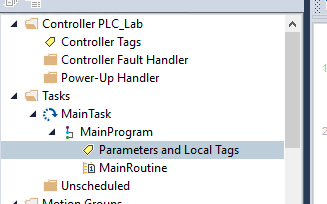
\includegraphics[width=3.2in]{BooleanTagCreation1}}
\caption{First step to creating a new boolean tag}
\label{fig:BooleanTagCreation1}
\end{figure}



\begin{figure}[h]
\centering
\textbf{Create new Boolean Tag}\par \medskip
\frame{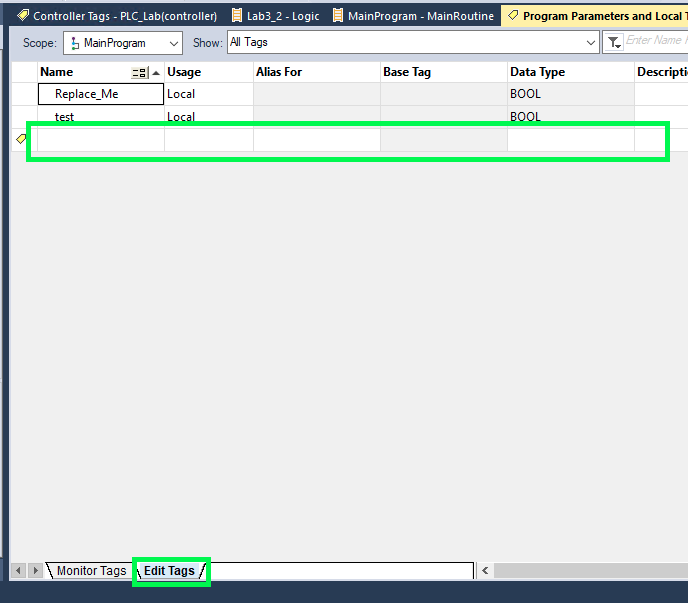
\includegraphics[width=3in]{EditTags}}
\caption{Second and Third step to creating a new boolean tag}
\label{fig:EditTags}
\end{figure}

\section{How to create a boolean tag}
\label{Section:BooleanTag}


To create another boolean tag to store the result of a boolean operation. Go to the left hand controller organizer menu. Under Main Program, double the item named Parameters and Local Tags. Refer to \figureautorefname \ref{fig:BooleanTagCreation1}.



Next, in the window that appears insure that you are on the edit tab of the parameters and tags window. In \figureautorefname \ref{fig:EditTags} you can see that the edit tab is in a green box for visibility at the bottom left. 

Finally, in the bottom entry in the list of tags enter the details for the tag that you are creating. The only two items that you should enter are the name and the datatype. The name must be a name that is not already taken and the datatype must be BOOL.


\input{Labs/PreLab3}
\chapter{Lab 3}
\setcounter{TASignatures}{0}
\setcounter{AsideCounter}{0}

\section{Introduction}
    \vspace{0.1em}

    \textbf{In this lab you gain experience with:}
    \begin{enumerate}
        \item Arithmetic instructions
        \item Compare instructions
        \item Implementing counters without using a counter instruction
        \item Implementing modulo functionality without using a modulo instruction
    \end{enumerate}

\subsection{Lab Files}

Go to iLearn and download the PLC and HMI files for this lab to the PC. Then download the PLC project to the PLC and the HMI application to the HMI. 

\subsection{Acceptable Instructions}

You may have previous experience with PLCs and that is great! However, you are only allowed to use the instructions that we have covered thus far in the lab. So, if you have experience already, consider it a challenge to restrict yourself to only use the instructions that have been covered thus far in lecture to solve the problem!

You are \textbf{not} allowed to use the modulo instruction, the counter instructions, the compute instruction, or the compare instruction. And as always you are \textbf{not} allowed to use the oneshot instruction (or any of the other rising/falling edge instructions).

\subsection{Lab agreement}

The planning of a program is often a very social activity, however the actual writing of the code is always an individual pursuit. In this class it is very much the same. Students are welcome to verbally assist each other, but each person is required to write their own code and personally complete each lab. In this way each student will gain valuable experience with programming PLCs. 

\textbf{The undersigned person guarantees that any and all work demonstrated to the TA in regard to this lab is a result of their own work with no unauthorized help.}

\signatureSlot{Student (Print \& Sign)}


\section{Transmission Makers of America}

This section corresponds to the \verb|Lab3_1| object in the Lab3 PLC file.
\\ 
\\
Transmission Makers of America (not a real company) is a tier 1 supplier of transmissions to automakers in the US. Their transmissions contain multiple gear packs which engage and disengage to provide the varying speed to torque relationship that cars require. 

Transmissions are difficult to manufacture because they require the gears to be meshed with very little backlash, and they must not be under a large amount of squeeze. One way to achieve such a precise fit would be to build every component absolutely perfectly... But that is extremely cost prohibitive. So, instead of counting on perfection, Transmission Makers of America use precisely sized shims to adjust the overall mesh depth of the gears, brilliant! 

The problem they are having is that the formula to calculate the correct size shim is quite complicated. Often when their employees calculate the necessary shim thickness, there are small math errors that render the transmission unusable. They have contracted you to code the fomula into a PLC and display the correct shim thickness on the HMI. They have already created the HMI and it has been provided to you so all you have to do is move the correct shim thickness into the \verb|Shim_Thickness| attribute from \tableautorefname \ref{Table:Lab3_1Attributes}. 

\aside{Backlash is the term used to describe the amount of separation between two gears. So, given gear A and gear B which are meshed together, the backlash is the rotation gear A can have \textbf{without} causing gear B to rotate.}

\aside{Tier 1 auto suppliers are those which are under contract to supply automotive components directly to automakers like GM, Ford, Toyota, etc.}

In reality, Transmission Makers of America only has shims in a few sizes. So, they use the shim that is closest in size to the ideal which will be calculated in the PLC. 

\begin{align}
\label{equ:Shim}
\tiny
\frac{Gear\_Diameter \cdot \sin{(Backlash)} \cdot Pinion\_Gear\_Depth}{(Drag\_Torque \cdot 20) + 3} - 2.32
\end{align}


\subsection{How should the logic work?}

That's for you to figure out.

\subsection{The Inputs and Outputs}

To access any of the signals listed in \tableautorefname \ref{Table:Lab3_1Attributes}, use the syntax \verb|Lab3_1.| followed by the attribute name. 

\begin{table}[h]
\centering
\caption{Attributes available in Lab3\textunderscore 1}
\label{Table:Lab3_1Attributes}
\begin{tabular}{c c c}
\toprule
Attribute Name & Data Type & Type\\
\midrule
\verb|Backlash| & Real & Output \\
\verb|Pinion_Gear_Depth| &  Real & Output \\
\verb|Gear_Diameter| &  Real & Output \\
\verb|Drag_Torque| &  Real & Output \\
\midrule
\verb|Shim_Thickness| & Real & Input\\
\bottomrule
\end{tabular}
\end{table}

Write the appropriate logic in the associated rung in the PLC file.

\TASignatureSlot



\section{Challenge - Modulo}

This section corresponds to the \verb|Lab3_2| object in the Lab3 PLC file.
\\ 
\\
Another weekly challenge from the competition for which you signed up! Write the logic necessary to calculate the modulo of two operands while only using the truncate, add, subtract, multiply, and divide instructions. Store the modulo of \verb|OperandA| and \verb|OperandB| in \verb|Calculated_Modulo|.

You may choose to create a new tag to store a temporary result. This is acceptable. If you need help creating a new tag, refer to \figureautorefname \ref{fig:BooleanTagCreation1_l3}. If the data you intend to store in the tag is not a boolean value \textbf{make sure that the datatype of the tag you create matches the datatype which you intend to store}. For this problem you will probably need to create a tag with datatype "Dint" or possibly "Real".

\aside{The modulo operation is typically denoted by the \% symbol.}

\aside{The TRN (truncate) instruction can be found in the Allen Bradley instruction set manual that is available. The truncate instruction removes the decimal portion of a number and leaves it whole without any rounding. ie. $TRN(6.1)=6.0$ and $TRN(6.99)=6.0$}

\subsection{How should the logic work?}

The modulo command calculates the remainder from a division operation. So, given \verb|OperandA| and \verb|OperandB|, calculate the remainder from $OperandA/OperandB$. As an example, if \verb|OperandA| is 5 and \verb|OperandB| is 3, then $OperandA \% OperandB = 2$. As a second example, if \verb|OperandA| is 13 and \verb|OperandB| is 6, then $OperandA \% OperandB = 1$. As a third example, if \verb|OperandA| is 14 and \verb|OperandB| is 7, then $OperandA \% OperandB = 0$. As a final example, if \verb|OperandA| is 5 and \verb|OperandB| is 2, then $OperandA \% OperandB = 1$. 

\aside{One of the powerful uses of the modulo operation, is it's ability to identify positive and negative numbers. Notice in the final example, $5\%2 = 1$. If the remainder of any number is non-zero after being divided by 2, then that number is odd.}

\subsection{The Inputs and Outputs}

To access any of the signals listed in \tableautorefname \ref{Table:Lab3_2Attributes}, use the syntax \verb|Lab3_2.| followed by the attribute name. 

\begin{table}[h]
\centering
\caption{Attributes available in Lab3\textunderscore 2}
\label{Table:Lab3_2Attributes}
\begin{tabular}{c c c}
\toprule
Attribute Name & Data Type & Type\\
\midrule
\verb|OperandA| & Dint & Output \\
\verb|OperandB| & Dint & Output \\
\midrule
\verb|Calculated_Modulo| & Dint & Input\\
\bottomrule
\end{tabular}
\end{table}

Write the appropriate logic in the associated rung in the PLC file.

\TASignatureSlot


\section{7 Boxes and Counting}

This section corresponds to the \verb|Lab3_3| object in the Lab3 PLC file.
\\ 
\\

The online retailer (You signed an non-disclosure agreement so you can't speak their name) which contracted you to automate their box moving process has now become a repeat customer! They now want you to implement a counting system to count how many boxes have been transferred to trucks.

They intend to use the box transfer counter as a means of keeping each shift on track. Each shift is intended to transfer 7 heavy parcels. However, some shifts are not hitting their goal. So, by having a counter on the screen to keep track of their progress, the retailer hopes to increase productivity. 

They also want you to reset the count when the shift leader hits the reset button on the HMI. Moreover, they want you to send a signal to the HMI when the shift goal is met. 

\subsection{How should the logic work?}

Each time \verb|Start_Transfer| goes from false to true, they want you to increment the value stored in \verb|Current_Count| to keep track of the number of boxes that have been transferred. They also want you to reset the counter to 0 whenever the \verb|Reset_Counter| tag is true. Finally, if the value in \verb|Current_Count| is greater than or equal 7, you should turn on the \verb|Shift_Goal_Met| bit.


\subsection{The Inputs and Outputs}


To access any of the signals listed in \tableautorefname \ref{Table:Lab3_3Attributes}, use the syntax \verb|Lab3_3.| followed by the attribute name. 

\begin{table}[h]
\centering
\caption{Attributes available in Lab3\textunderscore 3}
\label{Table:Lab3_3Attributes}
\begin{tabular}{c c c}
\toprule
Attribute Name & Data Type & Type\\
\midrule
\verb|Start_Transfer| & Bool & Output \\
\verb|Reset_Counter| & Bool & Output \\
\midrule
\verb|Current_Count| & Dint & Input\\
\verb|Shift_Goal_Met| & Bool & Input\\
\bottomrule
\end{tabular}
\end{table}

Write the appropriate logic in the associated rung in the PLC file.

\TASignatureSlot

\newpage
\begin{samepage}
\begin{figure}[h]
\centering
\textbf{Open Parameters and Local Tags}\par \medskip
\frame{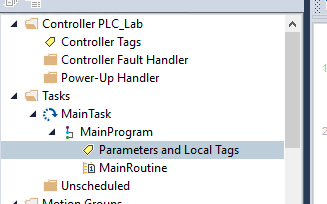
\includegraphics[width=3.2in]{BooleanTagCreation1}}
\caption{First step to creating a new boolean tag}
\label{fig:BooleanTagCreation1_l3}
\end{figure}



\begin{figure}[h]
\centering
\textbf{Create new Boolean Tag}\par \medskip
\frame{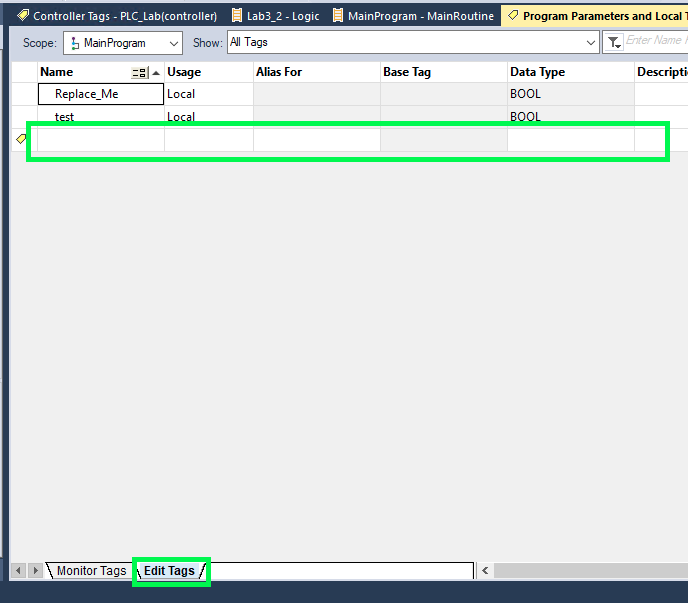
\includegraphics[width=3in]{EditTags}}
\caption{Second and Third step to creating a new boolean tag}
\label{fig:EditTags_l3}
\end{figure}

\section{How to create a boolean tag}
\label{Section:BooleanTag_l3}


To create another boolean tag to store the result of a boolean operation. Go to the left hand controller organizer menu. Under Main Program, double the item named Parameters and Local Tags. Refer to \figureautorefname \ref{fig:BooleanTagCreation1_l3}.



Next, in the window that appears insure that you are on the edit tab of the parameters and tags window. In \figureautorefname \ref{fig:EditTags_l3} you can see that the edit tab is in a green box for visibility at the bottom left. 

Finally, in the bottom entry in the list of tags enter the details for the tag that you are creating. The only two items that you should enter are the name and the datatype. The name must be a name that is not already taken and the datatype must be BOOL.
\end{samepage}
\chapter{Pre-Lab 4\&5}
\setcounter{TASignatures}{0}
\setcounter{AsideCounter}{0}

\section{Introduction}

Make sure to complete this pre-lab before your assigned lab time. You will not be allowed to begin working on your lab without having this complete.

\textbf{The coming lab will be extended across two lab times. So, you will not have a pre-lab next week!}

\section{Background}


In the coming lab we will be using timer and counter instructions. Be sure that you have watched the associated lecture and understand how the timer and counter instructions work as well as what their associated TIMER and COUNTER structures contain.


Each of the following problems are to be completed on paper. You are not expected to program these problems on PLC. You are expected to write neat ladder logic diagrams on paper.


\section{Problem 1}

Write the ladder logic necessary to implement a stopwatch in PLCfiddle. Submit your save URL for the PLC fiddle code in the ilearn submission folder. The stopwatch should have \verb|Start|, \verb|Pause|, and \verb|Reset| tags. The stopwatch must store the elapsed time in minutes and seconds in tags called \verb|Minutes| and \verb|Seconds| respectively. 

The stop watch should begin to accumulate when \verb|Start| is True. \verb|Pause|  becoming True should cause the accumulation to be paused. If the \verb|Start| button becomes True while the time accumulation is paused should cause the accumulation to continue \textbf{without} resetting the already accumulated time. The \verb|Reset| tag should both stop the accumulation of time and reset the currently accumulated time.



\section{Problem 2}

Write the ladder logic necessary to debounce a signal called \verb|input| and submit your save URL for the plc Fiddle code on ilearn. Debouncing is the name given to the process of making sure that a \textit{raw} signal has not been erroneously pressed or that noise has not been misconstrued as an True value. 

The approach is simple, use a TON timer (Called an On Delay Timer on PLC Fiddle) to detect when \verb|input| has been continuously True for 500ms.  When \verb|input| has been True for that period of time, turn on the signal \verb|input_debounced|. If \verb|input| changes from true to false, then \verb|input_debounced| should likewise change to false. 

Hint: The TON instruction will turn the .DN bit to True only after the rung in condition has been True for an amount of time greater than or equal to the timer preset value (In PLC fiddle, the .DN bit is called the Q bit). PLC fiddle timer presets are in seconds rather than milliseconds.


\section{Problem 3 - Read the Manual}

Read the lab manual. Then write a paragraph about the content and expectations in the lab manual which will convince the grader that you have in fact read the complete lab manual.
\chapter{Lab 4\&5}
\setcounter{TASignatures}{0}
\setcounter{AsideCounter}{0}

\section{Introduction}
    \vspace{0.1em}

    \textbf{In this lab you gain experience with:}
    \begin{enumerate}
        \item More arithmetic instructions
        \item More compare instructions
        \item Implementing counters using the counter instruction
        \item Timers
    \end{enumerate}

\subsection{Lab Files}

Go to iLearn and download the PLC and HMI files for this lab to the PC. Then download the PLC project to the PLC and the HMI application to the HMI. 

\subsection{Acceptable Instructions}

You may have previous experience with PLCs and that is great! However, you are only allowed to use the instructions that we have covered thus far in the lab. So, if you have experience already, consider it a challenge to restrict yourself to only use the instructions that have been covered thus far in lecture to solve the problem!

As always you are \textbf{not} allowed to use the oneshot instruction (or any of the other rising/falling edge instructions).

\subsection{Lab agreement}

The planning of a program is often a very social activity, however the actual writing of the code is always an individual pursuit. In this class it is very much the same. Students are welcome to verbally assist each other, but each person is required to write their own code and personally complete each lab. In this way each student will gain valuable experience with programming PLCs. 

\textbf{The undersigned person guarantees that any and all work demonstrated to the TA in regard to this lab is a result of their own work with no unauthorized help.}

\signatureSlot{Student (Print \& Sign)}


\section{7 Boxes and Counting... Again}

This section corresponds to the \verb|Lab5_1| object in the Lab5 PLC file.
\\ 
\\

The online retailer likes the work counting system you put in place to help them meet productivity. However, when their onsite technicians opened up the PLC code to make an adjustment, they were confused by what you had written. The online retailer has requested that you return to adjust your logic to use an Allen Bradley counter instruction instead of your hand implemented instruction. 

You are a bit annoyed by their request, but they are an important customer. So, you decided the best course of action is to put on a happy face and adjust your code.

\subsection{How should the logic work?}

You will have to create a tag of type COUNTER with the name \verb|Box_Counter|. To create a tag of type counter, refer to \figureautorefname \ref{fig:BooleanTagCreation1_l45}. The instructions there are for creating a boolean tag. So, the only difference will be that you will select the datatype COUNTER rather than BOOL.

After creating the counter tag, you will have to insert a count up (CTU) instruction into the logic. When you insert the CTU instruction, there are 3 available fields to customize the instruction to your particular needs. In \figureautorefname \ref{fig:CTU} notice the fields adjacent to the words counter, preset, and accum. 

\begin{figure}[h]
\centering
\textbf{CTU Instruction}\par \medskip
\frame{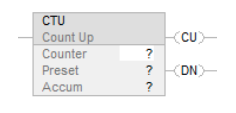
\includegraphics[width=3in]{CTU}}
\caption{Count up instruction}
\label{fig:CTU}
\end{figure}

The field beside the word counter is where you are to type the name of the COUNTER type tag you have created. The preset is the value which you would like to count up to. So, in this case you are counting up to the value 7. So, the preset should be 7. You can enter the value 7 directly into the preset field. 

The .DN bit which is part of the COUNTER type tag associated with the CTU instruction will be false until the counter value reaches the preset value. When the count value reaches the preset value, the .DN bit will become true. The .DN bit should be useful in deciding when to turn on \verb|Shift_Goal_Met|.

\aside{If you wanted to programmatically set the the preset value, you can do so by moving a value into the .PRE attribute which is a part of the COUNTER type tag associated with the timer instruction.}

To reset the counter, you will use a reset instruction (RES). This should be controlled by the \verb|Reset_Counter| signal.


\subsection{The Inputs and Outputs}

To access any of the signals listed in \tableautorefname \ref{Table:Lab5_1Attributes}, use the syntax \verb|Lab5_1.| followed by the attribute name. 

\begin{table}[h]
\centering
\caption{Attributes available in Lab5\textunderscore 1}
\label{Table:Lab5_1Attributes}
\begin{tabular}{c c c}
\toprule
Attribute Name & Data Type & Type\\
\midrule
\verb|Start_Transfer| & Bool & Output \\
\verb|Reset_Counter| & Bool & Output \\
\midrule
\verb|Current_Count| & Dint & Input\\
\verb|Shift_Goal_Met| & Bool & Input\\
\bottomrule
\end{tabular}
\end{table}

Write the appropriate logic in the associated rung in the PLC file.

\TASignatureSlot


\section{Challenge - The Maze Runner}

This section corresponds to the \verb|Lab5_2| object in the Lab5 PLC file.
\\ 
\\

This week the challenge activity is going to be a bit \textit{time} consuming (Pun!). This week the contest organizers decided that each contest will have to write a ladder logic program to guide a ball through a maze... automatically! The maze and the ball will appear on the HMI and you have to make the ball successfully navigate the maze!

\subsection{How should the logic work?}

The logic might seem tough at first glance but it's nothing you can't handle. The way to solve this problem is by writing a bit latch sequence. Each step in the sequence will control a timer and should turn on the appropriate direction control from \tableautorefname \ref{Table:Lab5_2Attributes}. You stay on that step until the timer completes. Then you move on to the next step. 
Hint: You will need one step for each change in direction that that the gold ball must make. ie. if there were 3 turns, then you would need a sequence with 3 steps. 

Hint: The length of time that each step should be on will be a bit of a guessing game. You'll have to figure out how long it takes for the ball to travel from where it starts to where you want it to be.

As a further requirement, when the \verb|Reset| becomes true you must unlatch all the steps in your sequence. When \verb|Go| becomes true the sequence should start and continue until the \verb|Reset| becomes true. Follow the approach to bit latch sequencing that has been discussed in lecture.

Hint: You will need to use timers to accomplish this task, obviously. You can complete it with either the TON timer or the RTO timer. 

\subsection{The Inputs and Outputs}

To access any of the signals listed in \tableautorefname \ref{Table:Lab5_2Attributes}, use the syntax \verb|Lab5_2.| followed by the attribute name. 

\begin{table}[h]
\centering
\caption{Attributes available in Lab5\textunderscore 2}
\label{Table:Lab5_2Attributes}
\begin{tabular}{c c c}
\toprule
Attribute Name & Data Type & Type\\
\midrule
\verb|Go| & Bool & Output \\
\verb|Reset| & Bool & Output \\
\midrule
\verb|Go_Up| & Dint & Input\\
\verb|Go_Down| & Bool & Input\\
\verb|Go_Left| & Bool & Input\\
\verb|Go_Right| & Bool & Input\\
\bottomrule
\end{tabular}
\end{table}

Write the appropriate logic in the associated rung in the PLC file.

\TASignatureSlot



\section{Double Challenge - Simple Waveform}

This week we have a rare double challenge. For the second challenge you are to use timers to make the waveform shown in \figureautorefname \ref{fig:SquareWave} appear in the axes on the HMI. However, the period of the square wave should be editable from the HMI. 

\begin{figure}
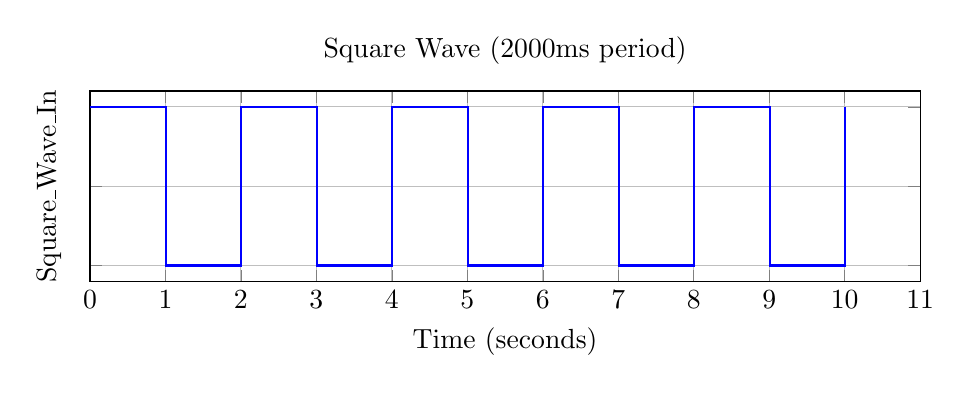
\begin{tikzpicture}
\begin{axis}[grid=both,xmin=0,width=\columnwidth,height=4cm,
title={Square Wave (2000ms period)},xlabel={Time (seconds)},ylabel=Square\_Wave\_In,
yticklabels={,,}]
\addplot+[thick,const plot, no marks,samples at={0,.01,...,10}] {(mod(x,2)>(2*0.5)?0:1)};
\end{axis}
\end{tikzpicture}
\caption{Square Waveform with a 2 second (2000 ms) period}
\label{fig:SquareWave}
\end{figure}

\subsection{How should the logic work?}

The axes shown on the HMI are continuously plotting the state of the \verb|Lab5_3| attribute called \verb|Square_Wave_In|. So, to make a squarewave appear on the axes, you must set \verb|Square_Wave_In| to true for an amount of time equal to one half of the period and then set the tag false for the same amount of time.

There is a field on the HMI that allows the user to edit the value stored in the \verb|Lab5_3| attribute called \verb|Period|. The value stored in this tag should be used as the period for your square wave.

\subsection{The Inputs and Outputs}

To access any of the signals listed in \tableautorefname \ref{Table:Lab5_3Attributes}, use the syntax \verb|Lab5_3.| followed by the attribute name. 

\begin{table}[h]
\centering
\caption{Attributes available in Lab5\textunderscore 3}
\label{Table:Lab5_3Attributes}
\begin{tabular}{c c c}
\toprule
Attribute Name & Data Type & Type\\
\midrule
\verb|Period| & Real & Output \\
\midrule
\verb|Square_Wave_In| & Bool & Input\\
\bottomrule
\end{tabular}
\end{table}

\TASignatureSlot


\begin{samepage}
\begin{figure}[h]
\centering
\textbf{Open Parameters and Local Tags}\par \medskip
\frame{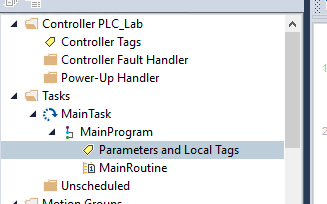
\includegraphics[width=3.2in]{BooleanTagCreation1}}
\caption{First step to creating a new boolean tag}
\label{fig:BooleanTagCreation1_l45}
\end{figure}



\begin{figure}[h]
\centering
\textbf{Create new Boolean Tag}\par \medskip
\frame{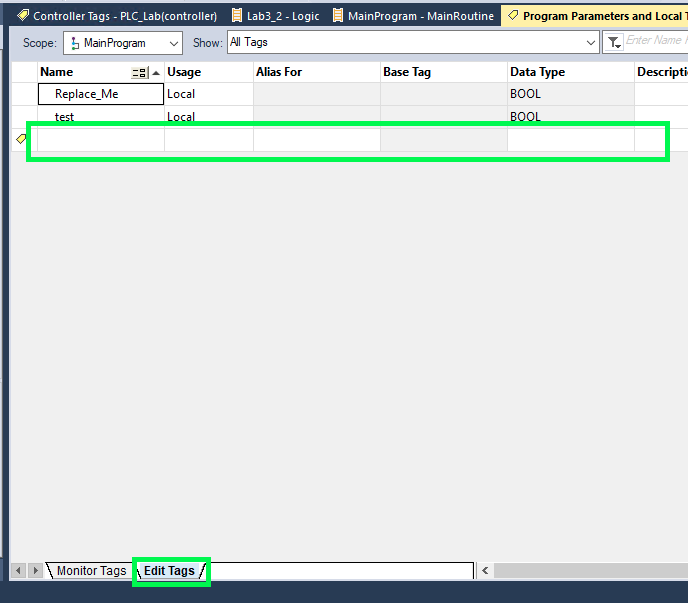
\includegraphics[width=3in]{EditTags}}
\caption{Second and Third step to creating a new boolean tag}
\label{fig:EditTags_l45}
\end{figure}

\section{How to create a boolean tag}
\label{Section:BooleanTag_l45}


To create another boolean tag to store the result of a boolean operation. Go to the left hand controller organizer menu. Under Main Program, double the item named Parameters and Local Tags. Refer to \figureautorefname \ref{fig:BooleanTagCreation1_l45}.



Next, in the window that appears insure that you are on the edit tab of the parameters and tags window. In \figureautorefname \ref{fig:EditTags_l45} you can see that the edit tab is in a green box for visibility at the bottom left. 

Finally, in the bottom entry in the list of tags enter the details for the tag that you are creating. The only two items that you should enter are the name and the datatype. The name must be a name that is not already taken and the datatype must be BOOL.
\end{samepage}

\chapter{Pre-Lab 6\&5}
\setcounter{TASignatures}{0}
\setcounter{AsideCounter}{0}

\section{Introduction}

Make sure to complete this pre-lab before your assigned lab time. You will not be allowed to begin working on your lab without having this complete.

\section{Background}


In the coming lab you will continue to use timer instructions, math instructions, and boolean logic. As an added component, you will also be making the HMI display screen for each of the portions of the lab. 

The coming lab will be extended across two lab times. So, you will not have a pre-lab next week!

\section{Problem 1}
Describe in detail the functionality for each of these HMI objects:
\begin{enumerate}
    \item Momentary Push Button
    \item Numeric Entry
    \item Numeric Display
    \item Text Box
    \item Multi-State Indicator
\end{enumerate}


\section{Problem 2}

Draw an HMI interface and state all necessary PLC tags required to set the speed of a centrifuge and display the current speed of the centrifuge. The operator should be able to enter a speed and then press a button to confirm that they want to set the centrifuge to the entered speed.

**If you are confused or feel that some information has not been given which is necessary, make assumptions to fill in the gaps and clearly state the assumptions that you have made (if any).

\section{Problem 3 - Read the Manual}

Read the lab manual. Then write a paragraph about the content and expectations in the lab manual which will convince the grader that you have in fact read the complete lab manual.
\chapter{Lab 6\&7}
\setcounter{TASignatures}{0}
\setcounter{AsideCounter}{0}

\section{Introduction}
    \vspace{0.1em}

    \textbf{In this lab you gain experience with:}
    \begin{enumerate}
        \item Editing HMI applications
        \item Sending information from the HMI to the PLC
        \item Displaying information from the PLC on the HMI
        \item More timers
    \end{enumerate}
    
    \textbf{You will also gain experience with the following HMI objects:}
    
    \begin{enumerate}
        \item Momentary Buttons
        \item Numeric Entry
        \item Numeric Display
        \item Text Boxes
        \item Multi-State Indicators
    \end{enumerate}

\subsection{Lab Files}

Go to iLearn and download the PLC and HMI files for this lab to the PC. Then download the PLC project to the PLC and the HMI application to the HMI. 

\subsection{Acceptable Instructions}

You may have previous experience with PLCs and that is great! However, you are only allowed to use the instructions that we have covered thus far in the lab. So, if you have experience already, consider it a challenge to restrict yourself to only use the instructions that have been covered thus far in lecture to solve the problem!

\subsection{Lab agreement}

The planning of a program is often a very social activity, however the actual writing of the code is always an individual pursuit. In this class it is very much the same. Students are welcome to verbally assist each other, but each person is required to write their own code and personally complete each lab. In this way each student will gain valuable experience with programming PLCs. 

\textbf{The undersigned person guarantees that any and all work demonstrated to the TA in regard to this lab is a result of their own work with no unauthorized help.}

\signatureSlot{Student}



\section{Editing the HMI Application}

In lab 0 you gained experience with downloading an existing HMI application to the HMI. At this point you should be familiar with how to set the IP address and download to the appropriate HMI. 

In this lab you will be editing an existing HMI application and programming the PLC so that both meet the requirements laid out in each of the lab exercises below. 

Each of the HMI objects necessary to complete this lab has been demonstrated in video lecture 6. Refer to the lecture if you are unsure how to create any of these objects. The video lecture also demonstrates the process to connect these objects with a tag in the PLC, create a runtime application, and download the runtime application to the HMI. The information in this section below is intended to reiterate what has already been demonstrated. 

\aside{The HMI interacts with the PLC by reading and writing values in PLC tags. When a button is pressed, the HMI typically writes a true value into some boolean tag. When the button is released, the HMI writes a false value into the tag. Similarly, when a number is entered into a numeric entry field, the HMI sets the value of an associated tag in the PLC to the value which was typed.}


\subsection{General Process to Developing an HMI application}

Here a general approach to developing an HMI application is given. This approach assumes that you have already have an HMI application file and with the settings chosen appropriately for the HMI to which the application will be downloaded. In this class, that will always be the case.

\subsubsection{Start by creating your tags in the PLC}
The HMI software is able to detect the available tags that are present in the PLC. This makes associating HMI objects with PLC tags easier. However, for the HMI software to accomplish this, the tags must already exist in the PLC. For this reason, \textbf{before you start developing the HMI application}, you should first create any tags that will be used in the HMI application and download the tags to the PLC. It is not necessary that all your PLC code be written, only that the tags you intend to use in the HMI are created in the project and downloaded.

\aside{In general it is best to keep your tags very organized. Often this involves using local tags only, with very few exceptions. However, in this introductory course, tag location is not emphasized.}

\subsubsection{Adjust the HMI communication setup}
For the HMI application and the PC software to see the tags which are in the PLC, you must complete the HMI communication setup as you typically would before downloading a project to the HMI at the beginning of lab. 


\subsubsection{Creating the object(s)}
After you have created and downloaded the tags you intend to use to the PLC and have successfully setup the communication for the HMI, it is time to begin making edits to the HMI application. At this point you should create the on screen objects that you need. 

\subsubsection{Connect the object to the desired PLC tag}
After you have created an object, \textbf{right click} the object and open the \textbf{properties menu}. Here, select \textbf{connections}. Depending on the object you have created, there may be multiple connection options. The options for a momentary pushbutton are shown in \figureautorefname \ref{fig:ConnectionMomentary}. 

In \figureautorefname \ref{fig:ConnectionMomentary} notice the column labeled "Tag" to the right of the center. The ellipses is clickable and gives a list of available tags.  

\begin{figure}[h]
\centering
\textbf{Connection options for Momentary Pushbutton}\par \medskip
\frame{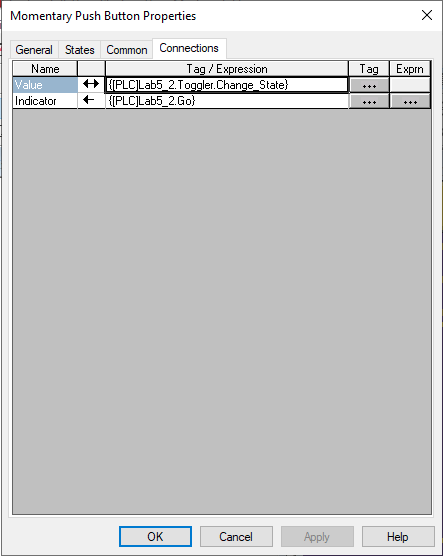
\includegraphics[width=3in]{ConnectionMomentary}}
\caption{Count up instruction}
\label{fig:ConnectionMomentary}
\end{figure}

After clicking the ellipses, a menu similar to the one shown in \figureautorefname \ref{fig:TagSelection} should appear. Select a folder on the left and the available tags in that folder will appear on the right. In \figureautorefname \ref{fig:TagSelection}, the folder called "Program.MainProgram" was selected. 

Note: Clicking the plus button beside a tag folder will show any nested folders. However, to see the tags in a folder, the folder itself must be highlighted.

Note: It may be that the HMI software (FactoryTalk View Studio) has not scanned the PLC to get the most updated list of available tags. If you don't see the tags you have created, click the Refresh All Folders button shown in the bottom left of \figureautorefname \ref{fig:TagSelection}. If you still can't find your tags, follow the steps below:

\begin{samepage}
\begin{itemize}
    \item Make sure you have downloaded the tags to the PLC
    \item Ensure that the PLC is in Run mode
    \item Make sure that the communication setup in the HMI has been completed
\end{itemize}
\end{samepage}

\begin{figure}[h]
\centering
\textbf{Tag selection}\par \medskip
\frame{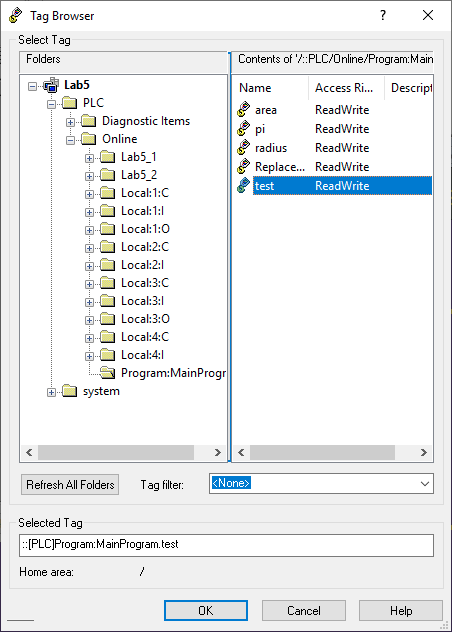
\includegraphics[width=3in]{TagSelection}}
\caption{Tag Selection}
\label{fig:TagSelection}
\end{figure}

\subsubsection{Create the Runtime Application}
When you have completed your HMI edits and are ready to download the application, it is time to create the runtime application. 

Go to the Application menu and select Create Runtime Application. In the dialog window that appears, select save. 

\subsubsection{Download the HMI application}
Finally, it is time to download the HMI runtime application. Use the transfer utility as you have previously to transfer the runtime to the HMI.



\section{Challenge - StopWatch}
(Notice that there is no associated object for this lab. You must create all the necessary tags and HMI objects to fulfill the requirements outlined in this exercise. Make sure that the HMI page you make looks professional.)
\\

Another weekly challenge from the competition for which you signed up! This week you will have to edit both the provided HMI and PLC files to accomplish the functionality.

Write a ladder logic program that will act as a stopwatch. Create a boolean tag called \verb|Start| that will act as the start button for the stopwatch. The \verb|Start| tag must be associated with a button labeled start on the HMI. Your PLC logic must calculate the time which has elapsed sense the \verb|Start| button was pressed. 

Further, you must create a pause button on the HMI that is connected to a boolean tag in the PLC that you must also create. The tag should be named \verb|Pause|. Your PLC ladder logic must implement pause functionality so that the stopwatch is paused after the \verb|Pause| signal becomes true and may be continued by pressing start again. 

Also, you must create a boolean tag in the PLC called \verb|Reset|. This tag must be associated with a button on the HMI with the same name. If the \verb|Reset| button is pressed then the timer should be reset to zero and stopped. 

Finally, the timer will track the elapsed time in milliseconds. You must take the elapsed time in milliseconds and convert it to seconds and minutes. The seconds and minutes should be displayed on the HMI.


\subsection{Hints}

The general logic has already been described.

You will need to create a tag of type TIMER. Create the tag and give it the name \verb|Stopwatch_TMR|. Use one of the two timer instructions that have been discussed in lecture. For information regarding the two timer instructions, refer to the Allen Bradley instruction manual on iLearn.

You will need to create the tags listed in \tableautorefname \ref{Table:Lab7_1Tags} in the PLC and use them appropriately in the HMI. You may create other tags as necessary.

\aside{The accumulated time is stored in the .ACC attribute of the TIMER tag. The value stored in the .ACC attribute is the elapsed time in milliseconds. To get the elapsed time in seconds and minutes is a matter of simple arithmetic.}

\subsection{The Inputs and Outputs}

To access any of the tags that you create, use the tag name without any prefix. This is different from the method used to access tags that were already provided in previous labs.

\begin{table}[h]
\centering
\caption{Tags you will create in Lab7\textunderscore 1\\ (Create others as necessary)}
\label{Table:Lab7_1Tags}
\begin{tabular}{c c}
\toprule
Tag Name & Data Type\\
\midrule
\verb|Start| & BOOL \\
\verb|Pause| & BOOL\\
\verb|Reset| & BOOL\\
\verb|Seconds| & Dint\\
\verb|Minutes| & Dint\\
\verb|Stopwatch_TMR| & TIMER\\
\bottomrule
\end{tabular}
\end{table}

Write the appropriate logic under the associated rung in the PLC file.

\TASignatureSlot



\section{Blinking Lights}
(Notice that there is no associated object for this lab. You must create all the necessary tags and HMI objects to fulfill the requirements outlined in this exercise. Make sure that the HMI page you make looks professional.)
\\

You have again been contacted by Transmission Makers of America to do some contract work for them. They want you to display a light (indicator) on the HMI and make the light (indicator) blink. 

A blinking light is actually a square waveform. So, they want to be able to enter the period in milliseconds of the blinking pattern. They also want to be able to enter the duty cycle in percentage on the HMI. So, if they enter 200 for the period and 50 for the duty cycle, it should produce a light blinking pattern like the one shown in \figureautorefname \ref{fig:Blink20050}. The Light has a "high" value on the graph, when the light is on, on the HMI.

\begin{figure}
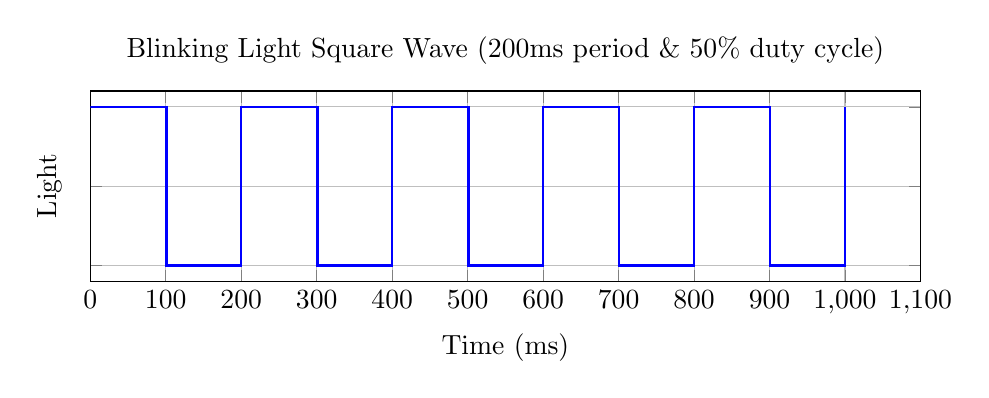
\begin{tikzpicture}
\begin{axis}[grid=both,xmin=0,width=\columnwidth,height=4cm,
title={Blinking Light Square Wave (200ms period \& 50\% duty cycle)},xlabel={Time (ms)},ylabel=Light,
yticklabels={,,}]
\addplot+[thick,const plot, no marks,samples at={0,1,...,1000}] {(mod(x,200)>(200*0.5)?0:1)};
\end{axis}
\end{tikzpicture}
\caption{Pattern on light with a 200ms period and 50\% duty cycle}
\label{fig:Blink20050}
\end{figure}

If the user were to type 400 for the period and 20 for the duty cycle, the PLC should cause the indicator on the HMI to blink in a pattern like that shown in \figureautorefname \ref{fig:Blink40020}.

\begin{figure}
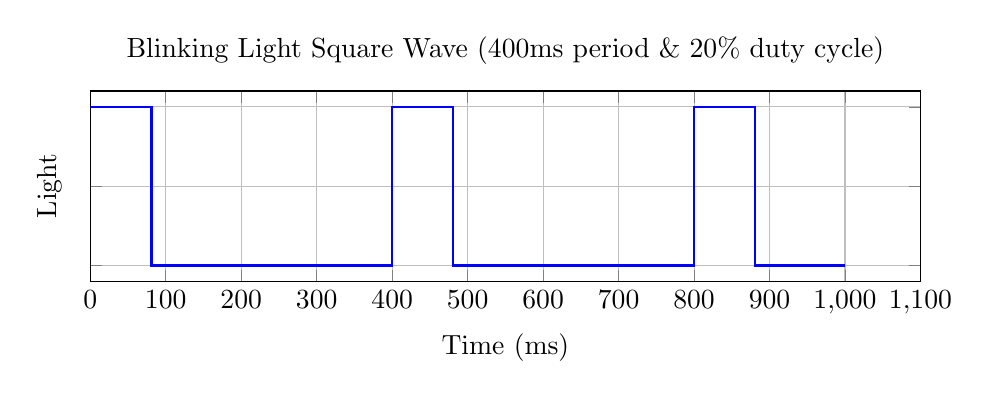
\begin{tikzpicture}
\begin{axis}[grid=both,xmin=0,width=\columnwidth,height=4cm,
title={Blinking Light Square Wave (400ms period \& 20\% duty cycle)},xlabel={Time (ms)},ylabel=Light,
yticklabels={,,}]
\addplot+[thick,const plot, no marks,samples at={0,1,...,1000}] {(mod(x,400)>(400*0.2)?0:1)};
\end{axis}
\end{tikzpicture}
\caption{Pattern on light with a 400ms period and 20\% duty cycle}
\label{fig:Blink40020}
\end{figure}

Note: In this exercise you decide what tags to create and what to name them. Make sure that you name them appropriately so that you (and others that may come behind you) know what the tags are meant to do.

\subsection{Hints}

To implement blinking lights, you will have to use timers. You will most likely need two timers. One for the on time, and one for the off time. Calculate the amount of on and off time using the period length and the duty cycle.

Problems like this are best attacked one step at a time. So, I would recommend the following decomposition:

\begin{itemize}
    \item Create the tag which you will associate with the hmi light in the PLC
    \item Create the multi-state indicator in the HMI, associate it with the PLC tag, and download the application
    \item Test the tag in the PLC by manually toggling it to see that the light blinks as it should
    \item Create timers and logic in the PLC to make the light blink
    \item Create the tags in the PLC for the desired duty cycle and blink period
    \item Write the logic to calculate the appropriate on and off time based on the period and duty cycle
    \item Test the duty cycle and period logic in the PLC manually by entering different values in the monitor tab of the tags menu
    \item Create numeric entry objects in the HMI and associate them with the duty cycle and period tags in the PLC
    \item Test the overall functionality
\end{itemize}

\TASignatureSlot



\section{C. A. L. See You Later.}
(Notice that there is no associated object for this lab. You must create all the necessary tags and HMI objects to fulfill the requirements outlined in this exercise. Make sure that the HMI page you make looks professional.)
\\


The grocery store manager has contacted you about doing some further work. They have been running into situations where they need a general purpose calculator available to all employees. They have purchased calculators in the past but they always manage to get lost. So, the manager wants you to add a calculator to the PLC and HMI that you have previously programmed. This way the calculator can't be lost!

The manager wants to be able to enter two operands on the HMI, \verb|operandA| and \verb|operandB|, and have the result of the calculation displayed in a third numeric display field on the HMI. The calculator must be able to multiply, divide, add, and subtract. There should be a button for each of these operations on the HMI that will apply the desired operations to the operands and display the result.

So, if a user enters 5 into the numeric entry field for \verb|operandA| and 3 into the numeric entry field for \verb|operandB| and then presses the button for multiply, the number 15 will be displayed in the numeric display field for the result. 

 
\subsection{From Functional Description to Code}


Typically, when a client specifies their desired functionality, the description will not be complete. Almost certainly they will not tell you how to implement the functionality they desire. So, in this problem, part of the exercise is figuring out what tags you will need to create in the PLC to make the desired HMI functionality possible. With that in mind, spend some time ensuring that you understand exactly how the calculator should work. Then consider how to accomplish the desired functionality using ladder logic and the HMI. After you have developed a plan, begin to program.

\TASignatureSlot



\section{What's the combination again?}
(Notice that there is no associated object for this lab. You must create all the necessary tags and HMI objects to fulfill the requirements outlined in this exercise. Make sure that the HMI page you make looks professional.)
\\


The grocery store manager had a second request. The store has a safe and every night all the large bills in the cash registers are removed and stored in the safe. But there are several department managers that need to be able to access the safe, some of which aren't very good at remembering the 7 number combination. The result is that every night the store manager is called and asked for the combination.

To fix this problem the manager has decided that they want you to add a screen to the HMI that will allow the department managers to type in a shorter pin number and press a button labeled ``Show Combo". After typing in the correct pin number and pressing the button, the safe combination will be displayed one number at a time, with each number being displayed for 3 seconds.

The manager has required that the pin number be 118. The safe combination is 3, 5, 8, 13, 21, 34, 55, 89. 

\aside{This problem has a set of things that must be done in the same order every time. These sequential functions are easier to implement if you use a structured bit latch sequence.}


\subsection{From Functional Description to Code}

Typically, when a client specifies their desired functionality, the description will not be complete. Almost certainly they will not tell you how to implement the functionality they desire. So, in this problem, part of the exercise is figuring out what tags you will need to create in the PLC to make the desired HMI functionality possible. With that in mind, spend some time ensuring that you understand exactly what the manager wants. Then consider how to accomplish the desired functionality using ladder logic and the HMI. After you have developed a plan, begin to program.

\TASignatureSlot
\chapter{Pre-Lab 8\&9}
\setcounter{TASignatures}{0}
\setcounter{AsideCounter}{0}

\section{Introduction}

Make sure to complete this pre-lab before your assigned lab time. You will not be allowed to begin working on your lab without having this complete.

\section{Background}


In the coming lab you will continue to use timer instructions, math instructions, and boolean logic. As an added component, you will also be making the HMI display screen for each of the portions of the lab. 


\section{Problem 1}
Read the lab 8\&9 manual and familiarize yourself with the program specifications. 

In the hints section that follows the program specifications there is a suggested approach to programming this lab. Follow the approach listed there, writing each of the specifications and the steps that you think will be involved. Then write the ladder logic (on paper) that you think will allow you to keep track of the average speed without keeping a history of past speeds. 


\section{Problem 2}

Draw an HMI interface and state all necessary PLC tags required to realize the HMI specifications laid out in the Lab 9 manual.

**If you are confused or feel that some information has not been given which is necessary, make assumptions to fill in the gaps and clearly state the assumptions that you have made (if any).

\section{Problem 3 - Read the Manual}

Read the lab manual. Then write a paragraph about the content and expectations in the lab manual which will convince the grader that you have in fact read the complete lab manual.
\chapter{Lab 8\&9}
\setcounter{TASignatures}{0}
\setcounter{AsideCounter}{0}

\section{Introduction}
    \vspace{0.1em}

    \textbf{In this lab you gain experience with:}
    \begin{enumerate}
        \item Developing HMI applications
        \item Applying course material to a real world problem
        \item Meeting functional software specification requirements
        \item Exceeding HMI design expectations
    \end{enumerate}

\subsection{Lab Files}

Go to iLearn and download the PLC and HMI files for this lab to the PC. Then download the PLC project to the PLC and the HMI application to the HMI. 

\subsection{Acceptable Instructions}

You may have previous experience with PLCs and that is great! However, you are only allowed to use the instructions that we have covered thus far in the lab. So, if you have experience already, consider it a challenge to restrict yourself to only use the instructions that have been covered thus far in lecture to solve the problem!

\subsection{Lab agreement}

The planning of a program is often a very social activity, however the actual writing of the code is always an individual pursuit. In this class it is very much the same. Students are welcome to verbally assist each other, but each person is required to write their own code and personally complete each lab. In this way each student will gain valuable experience with programming PLCs. 

\textbf{The undersigned person guarantees that any and all work demonstrated to the TA in regard to this lab is a result of their own work with no unauthorized help.}

\signatureSlot{Student}



\section{Challenge - Break week}

The challenge organizers decided to take some personal time off. So, there will be no challenge activity this week. It's a good thing too! You have a big contract coming up...



\section{Wamapoke County Contract}
(Notice that there is no associated object for this lab. You must create all the necessary tags and HMI objects to fulfill the requirements outlined in this exercise. Make sure that the HMI page you make looks \textit{very} professional.)
\\

While at an automation conference over the weekend, you met an interesting councilwoman from a small town in Indiana. Her name was Lesley Norpe (Or something like that). She was there looking to find someone to do some contract work for Wamapoke County, Indiana. She had heard positive things from your past customers and hired you on the spot. 

They want you to build a custom pressure road tube machine that will be used in assessing traffic flow between the urban and rural parts of the county. If you aren't sure what pressure road tubes are, watch the lecture. 


\subsection{Specifications for the Pressure Road Tube Machine}

\aside{Assume that all vehicles which pass through Wamapoke County only have two axles.}

\vskip1em
The pressure road tube machine must provide the following status data on the HMI:
\begin{enumerate}
    \item Speed of most recent vehicle
    \item Average speed of all vehicles sense the last reset
    \item Total vehicles sense the last reset
\end{enumerate}

\vskip1em
The pressure road tube machine HMI must allow the user to:
\begin{enumerate}
    \item Set the distance from tube 1 to tube 2
    \item Reset all status data with a single button press
\end{enumerate}

\vskip1em
The last thing that Wamapoke County has required is that the HMI be designed well. Specifically, they want all the required interface to be present (obviously), but they also want a nice depiction of a road with the pressure road tubes on the road. 

Further, the pressure road tubes in the HMI depiction should be clickable so that Lesley can test the machine without installing the tubes. Therefore, the tubes on the HMI will need to be buttons that are connected to the tag in the PLC which notifies your logic that a car is on a tube. 

\begin{samepage}
\subsection{Hints}

Problems like this are best attacked one step at a time. So, I would recommend the following decomposition:
\vskip1em
\begin{enumerate}
    \item [\textit{Program Spec}] 1. Be sure that you understand the specifications for the functionality.
    \item [\textit{Decomposition}] 2. Go through each of the required functions and create a list of steps that will be involved (ie. steps to count the number of vehicles, steps to reset all status data on button press).
    \item [\textit{Bottom-up}] 3. Sketch out the ladder logic necessary to complete each of the smaller steps that you have listed.
    \item [\textit{Implementation}] 4. Now that you have a fully developed plan, write the required ladder logic in the PLC.
\end{enumerate}

\vskip1em
As a final hint, do not try to keep a history of past speeds to calculate the average. Rather, figure out a way to calculate the new average using the current average, the current total vehicles, and the new, most recent speed.

\TASignatureSlot


\end{samepage}
\chapter{Pre-Lab 10\&11}
\setcounter{TASignatures}{0}
\setcounter{AsideCounter}{0}

\section{Introduction}

Make sure to complete this pre-lab before your assigned lab time. You will not be allowed to begin working on your lab without having this complete.

\section{Background}


In the coming lab you will be writing all the PLC logic and creating the HMI pages. Moreover, you will have to understand how state machines work as they will be used excessively in the coming labs.

The coming lab will be extended across two lab times. So, you will not have a pre-lab next week!

\section{Problem 1}

Using the process outlined in the lecture for coding a state machine, create a state machine that will toggle the value of a boolean tag called \verb|toggle_me|. The state machine should cause the value stored in \verb|toggle_me| to change when a rising edge occurs in the value stored in the tag called \verb|change|. 

Show each of the steps that are detailed in the lecture for programming a state machine.

As a hint, I suggest having the following states:
\begin{itemize}
    \item[] \verb|toggleMeIsOff_waiting_for_change_On|
    \item[] \verb|toggleMeIsOff_set_toggleMe_On|
    \item[] \verb|toggleMeIsOn_waiting_for_change_Off|
    \item[] \verb|toggleMeIsOn_waiting_for_change_On|
    \item[] \verb|toggleMeIsOn_set_toggleMe_Off|
    \item[] \verb|toggleMeIsOff_waiting_for_change_Off|
\end{itemize}

\section{Problem 2 - Read the Manual}

Read the lab manual. Then write a paragraph about the content and expectations in the lab manual which will convince the grader that you have in fact read the complete lab manual.


\section{Problem 3}

In the coming lab there will be a stoplight problem. Draw the state machine diagram and list all states, inputs, and outputs for the stoplight problem.

\chapter{Lab 10\&11}
\setcounter{TASignatures}{0}
\setcounter{AsideCounter}{0}

\section{Introduction}
    \vspace{0.1em}

    \textbf{In this lab you gain experience with:}
    \begin{enumerate}
        \item Programming State Machines in Ladder Logic
    \end{enumerate}

\subsection{Lab Files}

Go to iLearn and download the PLC and HMI files for this lab to the PC. Then download the PLC project to the PLC and the HMI application to the HMI. 

\subsection{Acceptable Instructions}

You may have previous experience with PLCs and that is great! However, you are only allowed to use the instructions that we have covered thus far in the lab. So, if you have experience already, consider it a challenge to restrict yourself to only use the instructions that have been covered thus far in lecture to solve the problem!

\subsection{Lab agreement}

The planning of a program is often a very social activity, however the actual writing of the code is always an individual pursuit. In this class it is very much the same. Students are welcome to verbally assist each other, but each person is required to write their own code and personally complete each lab. In this way each student will gain valuable experience with programming PLCs. 

\textbf{The undersigned person guarantees that any and all work demonstrated to the TA in regard to this lab is a result of their own work with no unauthorized help.}

\signatureSlot{Student}


\section{Simple State Machine}
Notice that there is no associated object for this lab. You must create all the necessary tags and HMI objects to fulfill the requirements outlined in this exercise. Make sure that the HMI page you make looks \textit{very} professional. 

This lab deals with state machines. In general you will need to fully define any state machine which you intend to program. However, in this part of the lab you are given the plain English description and the enumeration of states, inputs, and outputs.
\\

After successfully providing the pneumatic road tube machine to Wamapoke County, you were contacted again to do some additional work for Pawnee. They are adding a traffic light near town hall and would like you to program the light using an Allen Bradley PLC. 

As a constraint, they require any stoplight installations in Wamapoke county be programmed using state machines. They had an installation programmed by a fellow named Nadha Scolar that did not work well. It was observed that he did not use state machines. Therefore, state machines are now a required standard for all new Wamapoke stoplight controllers.

You may have never considered using state machines in a PLC before, so you are going back to your lair and develop a proof of concept as to how a state machine should work in a PLC.




\subsection{Plain English Description}

You are to program a state machine that will demonstrate how state machines work (similar to the one demonstrated in lecture with a few differences). The state machine is to have 3 states. They are to be called \verb|State1|, \verb|State2|, and \verb|State3|. \verb|State1| should be programmed to be the default state.

There are three inputs: \verb|transition1|, \verb|transition2|, and \verb|transition3|. The inputs are to be connected to buttons on the HMI. You are to draw the state machine diagram on the HMI and use it to show the current state. The transition buttons should be shown over top of the transition lines between the states. 

The outputs will be \verb|Show_State1|, \verb|Show_State2|, and \verb|Show_State3|. You are to use these outputs to show the current state on the state machine diagram on the HMI. Do not simply display the current state number. You are to display the current state in the same way demonstrated in the lecture practical. (This is to help you to continue getting better at HMI development.)

When the machine is in \verb|State1| and \verb|transition1| occurs, the machine should transition to \verb|State2|. When the machine is in \verb|State2| and \verb|transition2| occurs, the machine should transition to \verb|State3|. When the machine is in \verb|State3| and \verb|transition3| occurs, the machine should transition to \verb|State1|. 

\aside{In the practical example in the lecture for state machines, it was necessary to detect the rising edge of the change state button. This will \textit{not} be necessary here as each state has unique signals associated with the state transition.}


\TASignatureSlot



\section{Challenge - Toggle... Again}
Notice that there is no associated object for this lab. You must create all the necessary tags and HMI objects to fulfill the requirements outlined in this exercise. Make sure that the HMI page you make looks \textit{very} professional. 

This lab deals with state machines. In general you will need to fully define any state machine which you intend to program. However, in this part of the lab you should have already defined the components of the state machine in the pre-lab.


This week there will again be two challenges. The first of these challenges is to make a toggle program which is better than the unstructured toggle program you made previously in the semester.

This time, you are to make a toggle program using state machines. 

\subsection{Instructions}

In the pre-lab you were required to design the logic for a state machine that would act as a toggle program. Implement the logic in the PLC which you have designed. Fix any errors and then show your structured solution and its functionality to the TA.

\aside{By using a structured approach to the problem, you are no longer guessing and checking. Instead you have decomposed the problem into states and actions. These states and actions make the path to functionality clear. This is considerably better than the unstructured approach from earlier this semester.}

\TASignatureSlot





\section{Wamapoke Stoplight}
Notice that there is no associated object for this lab. You must create all the necessary tags and HMI objects to fulfill the requirements outlined in this exercise. Make sure that the HMI page you make looks \textit{very} professional. 

This lab deals with state machines. In general you will need to fully define any state machine which you intend to program. However, in this part of the lab you are given the plain English description. You will have to supply everything else.
\\

Now that you have experience coding state machines in an Allen Bradley PLC, you are ready to begin work on the stoplight. 


\subsection{Plain English Description}

The stoplight is to be a 4 way stoplight without a turn lane. So, there will be a total of 12 lights: 3 facing north, 3 facing south, 3 facing east, and 3 facing west. Refer to \figureautorefname \ref{fig:Intersection} for an illustration of the scenario. The yellow car is heading south and the city is to the north.

Notice cars which are traveling parallel to each other will have the same light displayed. So, the yellow car and any cars heading north will have the same color light. However, while the light is green for north and south traffic, any cars traveling east or west will have a red light. 

There are sensors in the road that detect cars which are waiting for the stoplight to become green. When a car is detected by the sensor continuously for 1 second, the green light shown to perpendicular traffic will immediately turn to yellow. The yellow light will be on for 10 seconds and then change to red. All directions of traffic will be red for 2 seconds, then the direction with the waiting car will change to green.

\begin{figure}[h]
\centering
\textbf{Simple Intersection}\par 
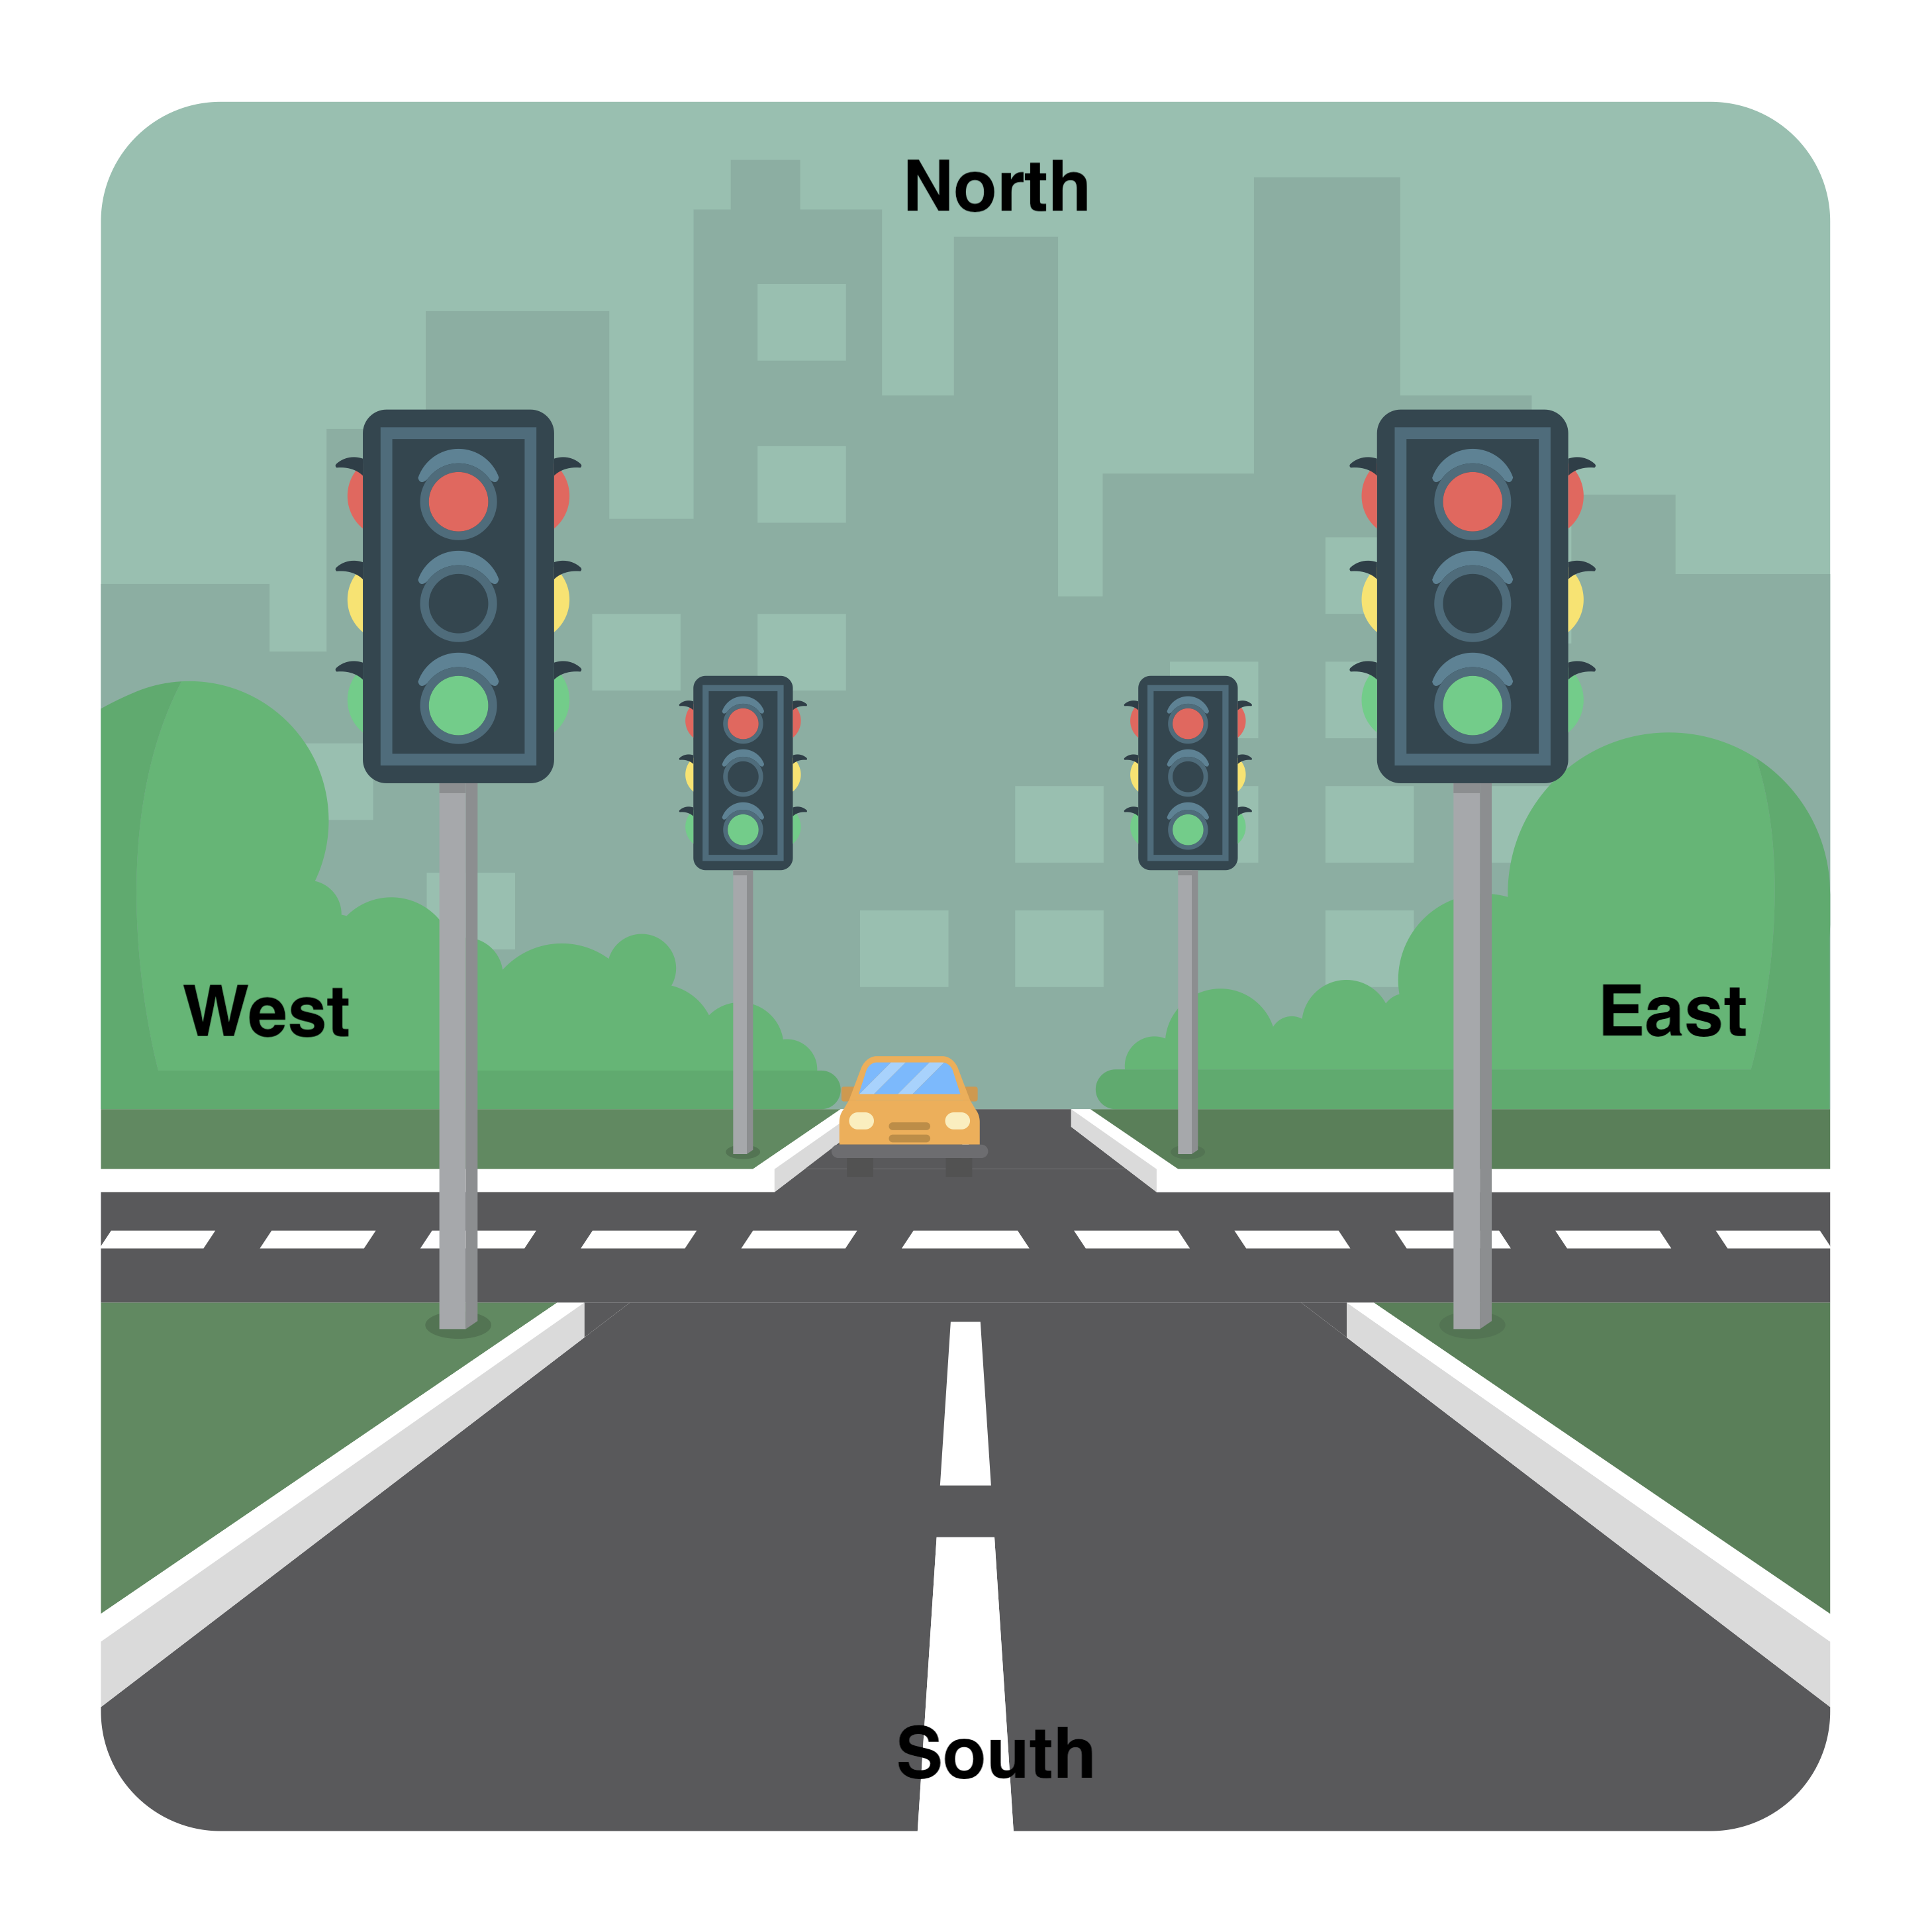
\includegraphics[width=3in]{Intersection}
\caption{Made available by Vecteezy.com}
\label{fig:Intersection}
\end{figure}


\begin{figure*}[t]
\centering
\textbf{The Final Problem - State Machine Diagram}\par
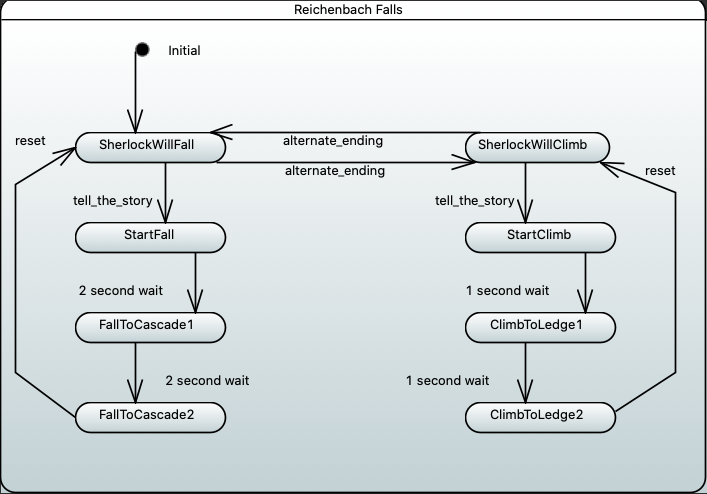
\includegraphics[width=6in, height=3in]{ReichenbachFallsStateDiagram}
\caption{State machine diagram for the final problem}
\label{fig:FinalProblemStateMachine}
\end{figure*}

\aside{The first 3 light traffic signal was invented in 1920 by William Potts, a police officer in Detroit. The older style of stoplight only had two lights and did not give drivers any warning before changing from green to red. This creates an obvious stopping problem if the driver is going at a high speed. By adding the amber light Potts resolved this issue.}

\subsection{Hint}

Each of the 12 lights should be outputs controlled by the current state. The sensors in the road will be the inputs. These sensors will have to be simulated on the HMI with push buttons. Don't forget that the sensor has to be on for an entire second before the car is considered to be waiting. The outputs should be shown on the HMI as multi-state indicators. 

Some state transitions will be based on timers...

\TASignatureSlot



\section{Challenge - The Final Problem}
Notice that there is no associated object for this lab. You must create all the necessary tags and HMI objects to fulfill the requirements outlined in this exercise. Make sure that the HMI page you make looks \textit{very} professional. 

This lab deals with state machines. In general you will need to fully define any state machine which you intend to program. However, in this part of the lab you are given the plain English description and the state machine diagram. You will have to supply everything else.

\subsection{Plain English Description}

The challenge organization has decided that this week will be the last challenge. They call it the Reichenbach machine. Reichenbach refers to the Reichenbach Falls in Switzerland. These falls were made famous in Sir Arthur Conan Doyle's Sherlock Holmes stories as the site of Holmes' alleged death.

The challenge is to have a depiction of the waterfall on the HMI. The depiction will need to include two cascades below Holmes' starting point and two ledges above. There is to be a button on the HMI which is labeled "tell the story". When the button is pressed, you are to depict Sherlock descending the 2 cascades to his doom. He should be on each of the cascades for 2 seconds.

However, there is to be another button labeled "alternate ending". This button will toggle the function of the "tell the story" button. After pressing the "alternate ending" button, the "tell the story" button should instead depict Sherlock climbing the two ledges above to secretly reach safety. When Sherlock climbs to safety, he spends 1 second on each of the two ledges. Finally there is to be a button labeled "reset" that will bring Sherlock back to the top of the falls.

Refer to \figureautorefname \ref{fig:FinalProblemStateMachine} for any additional information.

\subsection{How to make Sherlock move}

To be able to show Sherlock on the ledges and the cascades you will need to put a representation of him on the HMI. You may do this however, you see fit. However, you choose to represent Sherlock you will need to show him descending the cascades and ascending the ledges. 

It would be difficult to actually show him move (like the ball in the maze problem). Instead, it is easier to have multiple copies of your Sherlock representation on the screen at the various required locations. You can then control which of these Sherlocks is visible at a given moment. 

To control if something is visible programmatically, right click the object whose visibility you wish to control and select animation. In the animation dropdown, select visibility. In the menu that appears you can associate the objects visibility with the value stored in a particular tag in the PLC. If the tag contains the value \verb|True|, then the object is visible. Otherwise, it will not be visible on the HMI.

\TASignatureSlot
\chapter{Lab Final}
\setcounter{TASignatures}{0}
\setcounter{AsideCounter}{0}

\section{Introduction}
    \vspace{0.1em}

    \textbf{In this lab you gain experience with:}
    \begin{enumerate}
        \item Applying course material to a real world problem
        \item Meeting functional software specification requirements
        \item HMI object visibility
        \item HMI message display
    \end{enumerate}

\subsection{Lab Files}

Go to iLearn and download the PLC and HMI files for this lab to the PC. Then download the PLC project to the PLC and the HMI application to the HMI. 

\subsection{Acceptable Instructions}

You may have previous experience with PLCs and that is great! However, you are only allowed to use the instructions that we have covered thus far in the lab. So, if you have experience already, consider it a challenge to restrict yourself to only use the instructions that have been covered thus far in lecture to solve the problem!

\subsection{Lab agreement}

The planning of a program is often a very social activity, however the actual writing of the code is always an individual pursuit. In this class it is very much the same. Students are welcome to verbally assist each other, but each person is required to write their own code and personally complete each lab. In this way each student will gain valuable experience with programming PLCs. 

\textbf{The undersigned person guarantees that any and all work demonstrated to the TA in regard to this lab is a result of their own work with no unauthorized help.}


\subsection{Time}

Each student will have 110 minutes to complete the final. Completing the final in the time limit is not easy. It us meant to test how well each student has learned the course material and prepared for the final. Be careful to prioritize higher point value items to maximize your score!


\subsection{Lab Final Grading}

The lab final is different from the other labs throughout the semester. The lab counts as a single lab grade but is graded based on what portion of the lab you complete in this session. 

Refer to the grading rubric section for details.

\signatureSlot{Student}




\section{Winnipeg Industrial}
(Notice that there is no associated object for this lab. You must create all the necessary tags and HMI objects to fulfill the requirements outlined in this exercise. Make sure that the HMI page you make looks \textit{very} professional.)
\\

You have been contracted to program an industrial machine for Winnipeg Industrial. This machine is used to assemble the internal spline shaft in transmissions for certain American made vehicles. These shafts have several pieces that must be installed in a specific order. If the installation order is not correct, the transmission will fail.

Remember the loop that is present in typical industrial machines. An industrial control system commands an output based on a program, which causes some actuation in the environment. Then an instrument will detect the change in the environment and relay the detected change to the PLC via an input. 

Industrial machines that rely heavily on operator action are very common. The methodology used to program them is not very different than that used in automated machines. The primary difference is that a human operator will often act as the actuator and instrument. The PLC contains all the necessary instructions on how to assemble the product and shows the next instruction on the HMI screen. When the operator has completed the instructed action they press a button to signal the PLC. Then, the next command is displayed. In this way, the control system loop in the PLC is still sending commands via outputs and detecting the change in the world via inputs.

Winnipeg Industrial wants you to have one location to display instructions to the operator. If the operator takes more than 10 seconds to complete an instruction, then the HMI should flash an indicator with a 50/50 duty cycle and a 1 second period to get the operators attention and prompt them to continue the process. The flashing should stop once the operator has completed the overdue instruction.

When the operator has completed the instruction, they are to press a button on the HMI labeled \verb|ACKN| (short for acknowledge). The button should not be allowed to be pressed until the latest instruction has been visible for 1 second. Also, the next instruction should not be displayed until the button is released.

Winnipeg Industrial also wants you to keep track of how many parts have been completed. They also want you to track the average cycle time (The length of time elapsed after the operator acknowledges the ready to begin question until the process is completed). The part completed count and the average cycle time should be displayed on the HMI.

If any two consecutive cycles take more than 25 seconds to complete, set a boolean tag called \verb|manager_review| to true. This will tell the manager that they need to investigate the reason for the slow production. There should be a button on the HMI called manager login. When the button is pressed, the user should enter a code. If the code matches the manager's login code, an indicator showing state of \verb|manager_review| should be visible for 2 seconds. The manager login code is 7301863.

There should also be a button on the HMI called reset. This button will reset the state of \verb|manager_review|, the completed parts count, and the average cycle time.

Finally, all machines manufactured in the United States must have a category 0 stop mechanism. These are typically large red buttons labeled E-STOP. However, Winnipeg Industrial has applied to OSHA to receive a variance which allows them to have the E-STOP button on this machine be on the HMI. It is common to reset any running processes to an initial state when a category 0 stop occurs. So, you are required to have a red button on the HMI labeled E-STOP that will reset the instructions to the first step whenever it is pressed.

\aside{A category 0 stop is an action that when taken will remove all motive force. So, all power is removed from electrically powered motors, air pressure is removed from all possible cylinders, and the machine is generally rendered inoperable and ``safe".}

\subsection{List of instructions to assemble spline shaft}

\begin{itemize}
    \item Ready to begin?
    \item Place spline shaft in shaft retention nest
    \item Install pin bearing set 1
    \item Install pin bearing set 2
    \item Install clutch pack assembly
    \item Install ball bearings
    \item Install load plate
    \item Install snap ring
\end{itemize}

When the process is complete and the operator has released the \verb|ACKN| button, return to the first instruction so that the operator can begin on the next cycle.


\signatureSlot{TA Signature and Grade}

\begin{samepage}
\section{Grading Rubric}

\begin{enumerate}
    \item Make an attempt
    \begin{itemize}
        \item Everyone who shows up and tries gets these points (10 points)
    \end{itemize}
    
    \item Place to display operator instructions
    \begin{itemize}
        \item Are all the instructions displayed correctly and in the correct order consistently? (20 points)
    \end{itemize}
    
    \item Blinking indicator for taking too long to complete a step 
    \begin{itemize}
        \item Does the blink begin after 10 seconds? (4 points)
        \item Does the blink stop after the current instruction is complete? (3 points)
        \item Does it work for each of the instructions? (3 points)
    \end{itemize}
    
    \item \verb|ACKN| button
    \begin{itemize}
        \item Is the button only usable after 1 second? (3 points)
        \item Does the next instruction appear after releasing the button? (7 points)
    \end{itemize}
    
    \item E-STOP Button
    \begin{itemize}
        \item Does this button reset the process so that the first instruction is displayed? (10 points)
    \end{itemize}
    
    \item Completed parts count
    \begin{itemize}
        \item Does this correctly keep count of the number of completed parts? (10 points)
    \end{itemize}
    
    \item Average cycle time
    \begin{itemize}
        \item Is the average cycle time calculated and displayed correctly? (10 points)
    \end{itemize}
    
    \item Reset Button
    \begin{itemize}
        \item Does the reset button correctly reset the average cycle time and the completed parts count? (10 points)
    \end{itemize}
    
    \item Manager login and \verb|Manager_Review| indicator (hidden until manager login)
    \begin{itemize}
        \item Does the \verb|Manager_Review| tag correctly get set if two consecutive cycle times are longer than 25 seconds? (5 points)
        \item Is the \verb|Manager_Review| display indicator hidden until the manager logs in with the code? (3 points)
        \item Does the \verb|Manager_Review| display disappear after 2 seconds? (2 points)
    \end{itemize}
    
\end{enumerate}
\end{samepage}

\backmatter
\addcontentsline{toc}{chapter}{Index}
\printindex
\end{document}